%Preambolo per documento generico
%Per cambiare tipo di documento modificare
%il documentclass.

\documentclass[11pt]{article}
\usepackage[utf8]{inputenc}

%Mettere italian se si vuole scrivere in italiano
\usepackage[english]{babel}


%Aumento dell'interlinea
\usepackage{setspace}
\onehalfspacing

%Pacchetti per simboli matematici
\usepackage{mathtools}
\usepackage{amsfonts}
\usepackage{amsthm}
\usepackage{amssymb}
\newtheorem{theorem}{Theorem}
\usepackage{amsmath}
\usepackage{bm}


%Pacchetti per figure e tabelle
\usepackage{booktabs, caption, graphicx, subfig, float}
\captionsetup{tableposition=top,figureposition=bottom,font=small}

%Per inserire commenti in blocco
%Usage: \begin{comment} ... \end{comment}
\usepackage{comment}

%Definisce colori dei link nel testo e altri parametri
\usepackage{hyperref}
\hypersetup{
pdftitle={VSDProjectReport},%
pdfauthor={Carrarini,Kieffer,Tantucci,Wrona},%
pdfsubject={},%
pdfkeywords={},%
colorlinks=true,%
linkcolor=black,%
linktocpage=true,%
pageanchor=true,
citecolor=black
}

%Definisce in maniera simmetrica i margini di pagina
\usepackage{geometry}
\geometry{a4paper, top=3cm,bottom=3cm,left=3cm,right=3cm,%
			heightrounded}

%Per scrivere in maniera rapida norme e valori assoluti
%Usage: y = \abs{x} ; y = \norma{x}

%\DeclarePairedDelimiter{\abs}{\lvert}{\rvert}					%********************
%\DeclarePairedDelimiter{\norma}{\lVert}{\rVert}				%********************
%
%%Testo a caso
%%Usage: \lipsum[a-b] | Esempio \lipsum[1-10]
%\usepackage{lipsum}											%********************

%Cambia lo stile della pagina
%In alto a dx mette numero di pagina
%In alto a sinistra titolo e autore
\usepackage{fancyhdr}
\pagestyle{fancy}
\fancyhf{}
\rhead{\textit{\thepage}}
\lhead{\textit{Design and analysis of a KERS system for a F1 vehicle}}

%Per inserire codice nativo MATLAB e simili
%Usage: guardare sotto
\usepackage{fancyvrb}

\usepackage[dvipsnames]{xcolor}
\definecolor{sapred}{RGB}{130,36,51} %colore sapienza per i titoli

%%RIFERIMENTI IPERTESTUALI

%Tabelle e figure

% ...come si vede in Fig.~\ref{label}

%Equazioni

% ... dalla \eqref{label} si deduce che...


\begin{document}

\title{\textcolor{sapred}{Design and analysis of a KERS system for a F1 vehicle}\\\small{Vehicle System Dynamics Project}}
\author{Luca Carrarini\\Federico Kieffer\\Andrea Tantucci\\Andrea Wrona}
%Optional: data. Se non si inserisce il campo data
%LaTeX mette la data del PC automaticamente
%\date{}
\maketitle

\thispagestyle{empty}

\tableofcontents
\newpage

%Inizio dei capitoli
\section{Introduction}

The dependence of the transportation sector on non-renewable sources of energy as fossil fuels and the need for a rapid response to the global warming challenge has in the last two decades encouraged a strong effort for the development of fuel efficient vehicle propulsion systems. In this context, a particular attention has been devoted to the concept of regenerative breaking. 

A regenerative brake is a mechanism that reduces the vehicle speed by converting some of its kinetic energy into some other kind of useful forms of energy, such as mechanical, electrical or hydraulic energy \cite{a}. The core devices of regenerative brakes are therefore reversible energy conversion components like electric motors/generators and hydraulic pumps/motors. For example, an electric regenerative brake makes use of an electric motor that acts as a generator. This device, which is usually connected to the vehicle wheels trough a gear train, is indeed able to generate electrical energy thanks to the previously received kinetic energy that is associated to the vehicle at the end of any acceleration phase. 
A type of regenerative braking is called \textit{KERS}. 

KERS, which stands for \textit{Kinetic Energy Recovery System}, is an automotive system for recovering a moving vehicle kinetic energy under braking. The recovered energy is stored in a reservoir, as for example a flywheel, a battery or a super capacitor, for later use under acceleration \cite{b}. 

Embedding such a system in a vehicle allows several potential advantages. First of all, KERS systems may be included in the class of \textit{energy harvesting} devices \cite{c}, which are likely to have a consistent impact in the scenario of \textit{green technologies} and \textit{environment-friendly} solutions. In fact, the partial regeneration of the energy that is usually dissipated by the service brake in conventional systems may allow impactful fuel economy strategies, thus reducing the fossil fuel demand and the consequent green-house gases (CO2) emissions. 

Another important advantage that such a system introduces is the reduced service brakes wear. In fact, since during regenerative braking an electric/hydraulic motor is used to slow down the vehicle in place of the conventional disk brake, this component will as well benefit from a longer lifetime. 

\section{Implementation alternatives}

In this section, we give a description and a comparison of the principle KERS systems that have been proposed in the literature and on the market.

\subsection{Mechanical KERS}

\subsubsection{Architecture and working principle}

The Flywheel Hybrid System (FHS) is a type of KERS which consists of a rotating mass, or flywheel, as the energy storage device, a continous variable transmission system (CVT) to control and transfer the energy to and from the driveline and a clutch which connects this system to the primary shaft of the transmission (Fig. \ref{fig: FHS}). 

\begin{figure}[H]
\centering
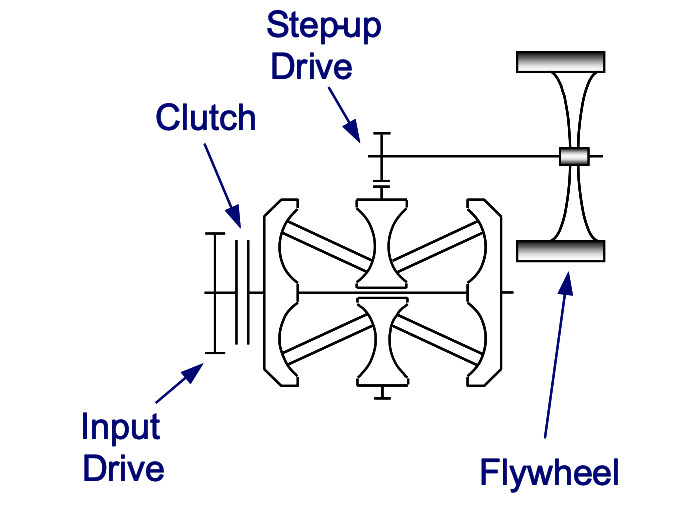
\includegraphics[width=.6\textwidth]{Images/State_of_the_art/Mechanical_KERS.png}
\caption{Schematic of Flywheel Hybrid System}
\label{fig: FHS}
\end{figure}

When the brakes are applied or the vehicle decelerates, the clutch connecting the flywheel system to the driveline/transmission is engaged, causing energy to be transferred to the flywheel via the CVT. 

The use of the CVT guarantees a smooth transfer of energy thanks to the fact that it has an infinite number of gear ratios between the maximum and minimum value of the speed. The Toroidal CVT must continuously adjust the ratio between the speed of the vehicle and the rotation of the flywheel. Any change in the CVT ratio can be viewed as the transfer of kinetic energy between the flywheel inertia and vehicle.

The flywheel stores this energy as rotational energy and can rotate up to a maximum speed of (usually) $60000$ [rpm]. When the vehicle stops, or the flywheel reaches its maximum speed, the clutch disengages the flywheel unit from the transmission allowing the flywheel to rotate independently. Whenever this stored energy is required, the clutch is engaged and the flywheel transmits this energy back to the wheels, via the CVT. To optimize efficiency, the flywheel runs in a high vacuum and is enclosed within a housing that provides containment in the event of failure.

The major function of the vacuum chamber is to minimize the air resistance as the flywheel rotates. Without the vacuum chamber, the friction caused by air resistance is enough to cause significant energy losses and heat the carbon fibre rim to its glass transition temperature. In Fig. \ref{fig: Flywheel} we can see the design of a flywheel.

Another important part of the system is the bearings on which the flywheel is mounted. Magnetic bearings have replaced mechanical bearings as they greatly reduce losses due to friction. Further magnetic bearings are able to operate in vacuum which leads to even better efficiency. The magnetic bearings support the flywheel by the principle of magnetic levitation. It is important that the bearings are able to operate inside a vacuum because the flywheel in a flywheel-based KERS must rotate at high speeds for maximum efficiency. The best performing bearing is the high-temperature super-conducting (HTS) magnetic bearing.

\begin{figure}[H]
\centering
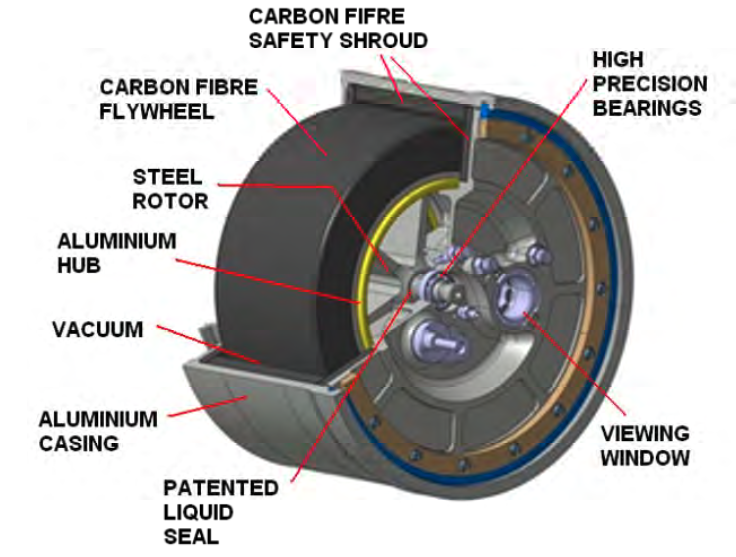
\includegraphics[width=.6\textwidth]{Images/State_of_the_art/Flywheel_Components.png}
\caption{Section of the flywheel}
\label{fig: Flywheel}
\end{figure}

There is also a step--up gearing system consisting of epicyclic gears, connected between the CVT and the flywheel unit. This system is used to reduce the speed of the flywheel to a manageable one outside the vacuum chamber, in order to have a smooth transfer of energy to the CVT.

The clutch instead is used to couple the flywheel hybrid system to the transmission. It engages the system while the flywheel is accelerating from rest and disengaging while the flywheel is rotating and the vehicle is at rest. Torque is transferred through clutch between the flywheel and vehicle. Hence, the power transmitted in the flywheel system can be controlled by a clutch that could continuously manipulate the torque.

\subsubsection{Advantages, disadvantages and fields of application}

The advantages include high efficiency, low fuel consumption, and low cost compared to electric hybrids. Although the system has a few drawbacks, most of it can be outweighed by the benefits. 

One main advantage of this KERS system is its weight. Due to the lightweight design of the flywheel and accompanying components, the additional weight is insignificant when analyzing fuel efficiency. Moreover, the system is contained in a compact package, making it easy to incorporate into the rear of a vehicle. Another advantage is the ability of the flywheel to store energy efficiently. This is because there is no transformation of energy from one form to another which greatly reduces energy losses in the system. Tests have proven that flywheel--based KERS can recover and store over $70\%$ of vehicle energy. Probably the only losses that occur in the system might be due to friction and air resistance to the flywheels rotation. However, the magnetic bearings and vacuum chamber mentioned previously have been developed to minimize these effects. Cars with a flywheel based energy recovery system, though significantly more expensive than cars without this system, have more power and better fuel efficiency. It has been proved that the system could reduce fuel consumption by as much as $20$\% and give a four-cylinder engine acceleration like a six-cylinder unit.

The system has low maintenance costs and it reduces break wear. As with any technology, the flywheel KERS system has its shortcomings as well. The flywheels found in a kinetic energy recovery system can store up to $400$ kJ of energy, which means that failure while rotating at $60000$ [rpm] could cause immense amounts of damage. The flywheel--based KERS is not designed to be a stand-alone source of power for a vehicle, like batteries are in electric cars. It is designed for temporary energy storage that is to be used frequently and in smaller amounts. Its purpose is to reduce fuel consumption by providing additional power during the acceleration of a vehicle. Periods of acceleration, especially from a stop, are when the efficiency of the vehicle is at its lowest.


\subsection{Electric KERS}

Electric KERS is a type of KERS which makes use of batteries or/and supercapacitors as storage system. This regenerative braking system can be used both in the case of internal combustion engine, electric vehicle and hybrid vehicle.

\subsubsection{Architecture and working principle}

There are different implementations in literature of electric KERS (e-KERS) and each architecture is more suitable for particular application. In Fig.~\ref{ekersdrivetrainuc} e-KERS with supercapacitor as principal and unique storage system is described. The scheme is composed by: the supercapacitor (SC) which is the energy storage part of the system; it is electrically interfaced to the motor-generator unit (MGU) through power converter (PC). MGU is connected to drive shaft. 

\begin{figure}[H]
	\centering
	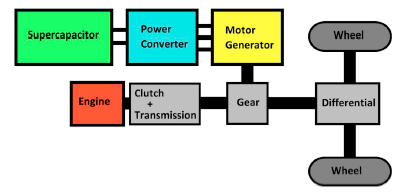
\includegraphics[width=.6\textwidth]{Images/State_of_the_art/Electric_KERS_uconly.PNG}
	\caption{Drivetrain layout with e-KERS}
	\label{ekersdrivetrainuc}
\end{figure}
 
\begin{figure}[H]
	\centering
	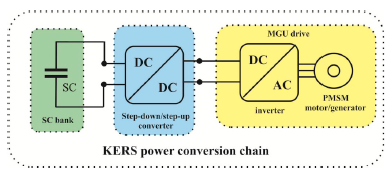
\includegraphics[width=.6\textwidth]{Images/State_of_the_art/Electric_KERS_scheme_uconly.PNG}
	\caption{E-kers scheme}
	\label{ekersschemeuc}
\end{figure}

There exists also the dual of this implementation which is the one in which there are only batteries used as storage system. These two implementations have several limitations. SC as single energy storage element can be used only when large spaces and weight were allowed (i.e. electric city rail, hybrid city bus). Batteries have high energy density(Li-ion batteries, that are the most installed batteries on electric vehicle, have specific energy density around $75–200$ [Wh/kg]) but low power density. For automotive applications, specifically in hard braking and traction maneuvers, batteries present several weaknesses related to the chemical reactions taking place while charging/discharging. 

Li-Ion batteries cannot respond to high-dynamic power profiles resulting from an acceleration or a regenerative braking since charge transfer occurs through reduction and oxidation reactions. These profiles, if happened, will overstress the batteries which negatively affect the longevity of their lifespan. It is convenient to implement in the system a storage element characterized by its ability to provide the necessary power required by the traction and braking systems. This secondary storage element will substitute the battery during extreme power demand. Among all the existing storage elements, the supercapacitors are potential candidates to meet those requirements. This element has high power density and high cycle life. On the other hand, it presents a low energy density, a high acquisition cost and a high self-discharge. The hybrid energy storage system (HESS) will combine the high energy density storage element (Li-Ion battery), known as primary storage element, and the high power density storage element (supercapacitor). HESS implementation is described in Fig. \ref{ekersschemehybrid}

\begin{figure}[H]
	\centering
	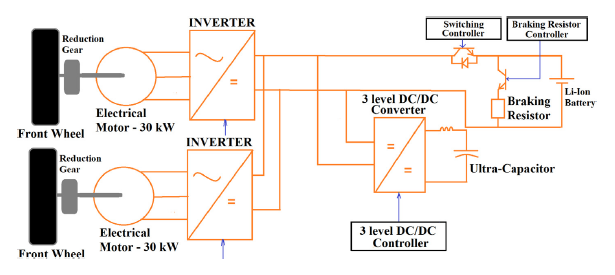
\includegraphics[width=.6\textwidth]{Images/State_of_the_art/Electric_KERS_scheme_hybrid.PNG}
	\caption{Hybrid e-kers scheme}
	\label{ekersschemehybrid}
\end{figure}

It is possible to see in Fig. \ref{ekersschemepowerflow} the power flow from wheels to storage system during brake phase.

\begin{figure}[H]
	\centering
	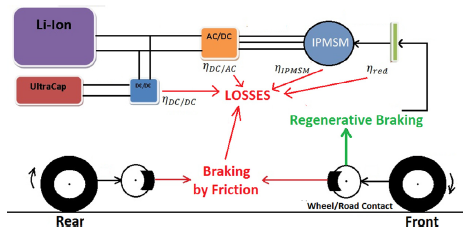
\includegraphics[width=.6\textwidth]{Images/State_of_the_art/Electric_KERS_powerflow.PNG}
	\caption{Hybrid e-kers scheme}
	\label{ekersschemepowerflow}
\end{figure}


\subsubsection{Advantages, disadvantages and fields of application}

It is possible to evaluate and to compare electrical energy storage system by using some performance metrics like the cycle efficiency, the cost per unit capacity(\$/[kWh] or \$/[kW]), specific energy ([Wh/kg]), specific power ([W/kg]) ,energy density ([Wh/l]), power density ([W/l]), cycle life. 

The battery has shorter cycle life due to unavoidable chemical deterioration. No single type of electrical energy storage element can simultaneously fulfill all the desired characteristics. There will be a need to combine higher energy density insured by the battery, as primary source, with a higher power density energy storage elements, like ultracapacitors or flywheel. This means that the best e-KERS implementation is the hybrid one which makes use of primary and secondary source. The use of supercapacitor as unique storage solution in electric vehicles remains limited since their energy density cannot compete with batteries. 

It is possible to use only supercapacitors as storage system if a low driving range can be accepted and if there is enough space available to install supercapacitors and when there are no weight constraints as in the case of electric city rail or hybrid city bus, where energy saving of about $40\%$ were obtained. Both HEV and FCHEV usually implement electric KERS, exploiting the main storage system used for the traction in conjunction with supercapacitors, which allow a reduction of batteries intervention during vehicle regenerative braking or startup, thus enhancing batteries life cycle and maintaining their capacity performance. Regenerative braking has been intensively studied and implemented on hybrid electric vehicles (HEV) and fuel cell hybrid electric vehicles (FCHEV) because the presence of powerful electric machines (generator and motor) interfaced to high capacity energy storage as batteries easily allows to convert and store vehicle kinetic energy into electric energy. Stored energy can be employed for vehicle propulsion or for electronic components supply.  Stationary flywheels have important dimensions and excessive weight. On--board flywheels need space in the bogie requiring more space than ultracapacitors. After the diffusion of UCs, the use of flywheels in electrified railways has been reduced because of the superior properties of UCs in terms of maintenance, weight and size.

Other authors conclude that flywheel ensures a steady voltage and power level, which is independent of load, temperature and state of charge. In fact, the combination battery/flywheel can achieve better performance, regarding voltage fluctuation, than other types of combinations (battery/UC or UC/flywheel). Unlike electrified vehicles, internal combustion engine vehicles are not equipped with generator, electric motor and batteries of adequate power and capacity to allow the conversion of the vehicle kinetic energy into electric energy. For this reason, the kinetic energy recovery systems successfully tested for ICEV application are mainly based on mechanical and hydraulic energy storage devices. Unfortunately, the energy recovered through the flywheel cannot be stored for a long time, due to mechanical and fluid dynamics friction on the flywheel.
 

\subsection{Hydraulic KERS: Series Hydraulic Hybrid systems}

Series Hydraulic Hybrid Systems(SHH) represent a type of KERS that makes use of hydraulic accumulators as energy storage units. Unlike the older \textit{parallel} implementations, the \textit{series} architecture is characterized by the fact that prime-mover and vehicle speeds are entirely decoupled through a continuously variable hybrid hydraulic transmission. In other words, the conventional mechanical driveline is completely removed.

\subsubsection{Architecture and working principle}

The system (Fig.~\ref{SHH_scheme}) is made of four principal components \cite{d} the working fluid (usually oil), the ICE, hydro-pneumatic accumulators and pumps/motors, which are often variable displacement axial piston machines.

\begin{figure}[H]
\centering
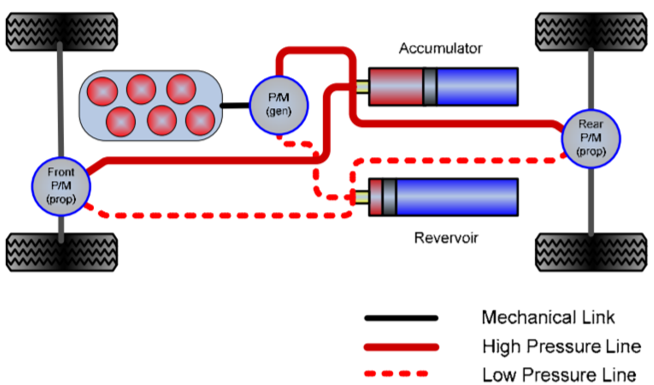
\includegraphics[width=.6\textwidth]{Images/State_of_the_art/Hydraulic KERS.png}
\caption{SHH scheme for a 4x4 vehicle}
\label{SHH_scheme}
\end{figure}

The IC engine is mechanically coupled to the hydraulic pump/motor designated as P/M(gen). The P/M(gen) is used as a motor only when starting the engine. In all the other working conditions, the fluid pumped by P/M(gen) flows towards the P/M(prop-s) and the high pressure accumulator. Traction pumps/motors (P/Mprop-s) are connected to the wheels through a differential to provide propulsion. The pump/motor is a reversible energy conversion component. In particular, operating the P/M(prop) in the motor mode propels the vehicle, while regenerative braking requires switching to the pump mode. During the breaking phase, the hydro-pneumatic accumulator allows energy storage: as the P/M(prop), working as a pump, transfers the hydraulic fluid from the reservoir into the accumulator, the pressure of the gas sealed inside it increases, thus storing energy \cite{e}. 

In the accumulator (Fig.~\ref{hydraulic_accumulator}), a bladder is used to separate the working fluid from the pressurized inert gas (e.g. nitrogen), which can be thus treated as a closed system. In a later acceleration event, the energy stored in the high pressure fluid contained in the accumulator is used, together with an amount delivered by the P/M(gen), to provide torque to the wheels. The pressure difference between the accumulator and the reservoir determines the maximum torque available from the hydraulic motor. In this phase, the working fluid is at least partially returned to the reservoir. 

\begin{figure}[H]
\centering
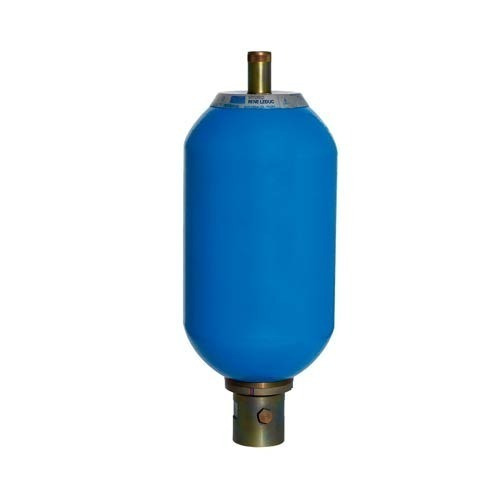
\includegraphics[width=.4\textwidth]{Images/State_of_the_art/Hydraulic Accumulator.jpg}
\caption{Commercial bladder-type hydraulic accumulator}
\label{hydraulic_accumulator}
\end{figure}

The reservoir is structurally similar to the accumulator but the gas that it contains is kept at low pressures and serves primarily to assist the transfer of fluid to-and-from the accumulator, with a minimal impact on the overall energy conversion. 

\subsubsection{Advantages, disadvantages and fields of application}

In contrast to its electric counterpart, fluid power technology is characterized by a higher power density and lower energy density \cite{f}. Energy density, which is also known as specific energy, represents the amount of energy that can be stored in a given mass of the system. On the other hand, energy density does not give information on how quickly this energy can be used: this knowledge is contained in the system power density, which describes the rate at which its energy can be outputted. 

Moreover, since they release their energy more quickly, higher power density systems can also recharge more quickly. This feature makes hydraulic hybridization particularly interesting for applications with high and fast power transients. In particular, utilization of hydraulic propulsion and energy storage components can offer significant advantages for the heavy vehicles that require frequent start-stop operations, such as city buses, delivery vehicles and refuse trucks. It is worth noticing that, in those fields of application, the stored energy is not necessarily limited to aid subsequent acceleration events, but can potentially represent a power source for the activation of ancillary equipment, as for example the compacting and packing mechanisms of refuse trucks. In addition, hydraulic KERS are also likely to have a longer operating life than battery-powered systems.  

Another remarkable advantage of those systems is their high energy conversion efficiency: the state-of-the art bladder type accumulators with elastomeric foam can reach a round-trip efficiency of about 95\%. Once again, the combination of high efficiency and high charging-discharging rates enables particularly effective regeneration and re-use of hydraulic energy in heavy vehicles.

The main disadvantage of hydro-pneumatic KERS is represented by their high weight, which is mainly due to the presence of the working fluid and accumulators. This causes the specific energy of those systems to be relatively low. As a result, hydraulic hybrid systems encounter important limitations where consistent levels of power are required for extended periods at near constant speeds, such as in long-distance cruising.
Additional costs, which may represent 10–15\% of the total for the vehicle, is undoubtedly a further important drawback.

\subsection{Hydro-electric KERS}

This type of KERS is called also HESS (\textit{hydro electric synergy system}). It is an alternative of the above described pure hydraulic KERS, because of the introduction of a second energy storage system.

\subsubsection{Architecture and working principle}

The HESS is composed by two main parts:

\begin{enumerate}
	\item \textbf{Hydraulic System}. It is the main energy recovery system, characterized by high power density. It includes:
	\begin{itemize}
		\item Pump or motor (Fig.~\ref{hydraulic_pump}) (depending on the usage phase). During the acceleration phase, it behaves like a motor, providing torque to the shaft, whereas during deceleration it behaves like a pump, storing the fluid from the reservoir into the high--pressure accumulator;
		\begin{figure}[H]
			\centering
			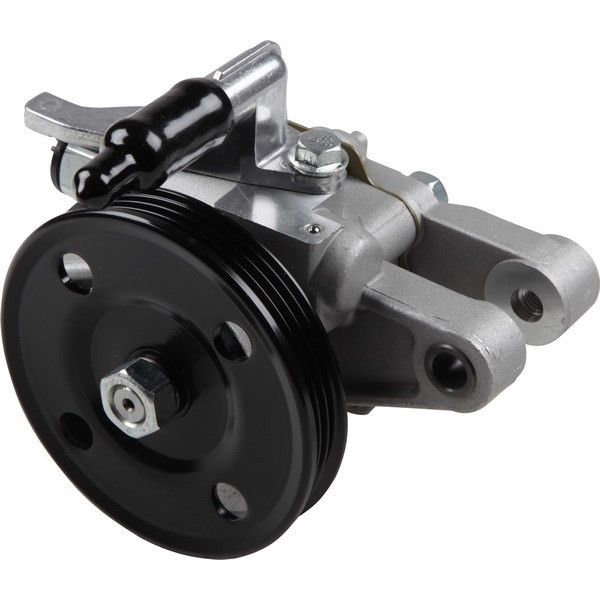
\includegraphics[width=.3\textwidth]{Images/State_of_the_art/Hydraulic Pump.jpg}
			\caption{Commercial hydraulic pump}
			\label{hydraulic_pump}
		\end{figure}
		
		\item Accumulator;
		\item Reservoir.
	\end{itemize}
	\item \textbf{Electric System}. It constitutes the secondary energy recovery system, characterized by a high energy density. It is used only when a high amount of power is requested by the user or when there is a fault on the hydraulic machinery. This allows to maintain the battery around its optimal state of charge (SoC). It includes:
	\begin{itemize}
		\item Battery. Usually a nickel--metal--hybrid (Ni--MH) one is used. It is linked to the electric motor (EM) through a DC/DC converter;
		\item Electric motor. It can be used as a motor or as a generator, depending on the usage phase;
		\item DC/DC converter.
	\end{itemize}	
\end{enumerate}

A typical realization scheme for the HESS can be seen in Fig.~\ref{HESS scheme}.

The overall system is driven by a centralized controller which decides the action to be performed depending on the nature of the torque applied by the human (positive if the vehicle is accelerating). The primary task of the control action, as in all KERS, is to maximize the fuel economy.

\begin{figure}[H]
\centering
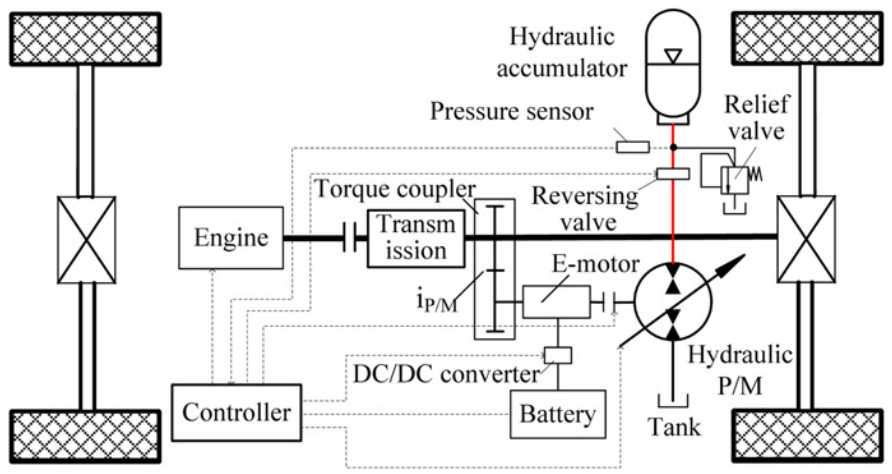
\includegraphics[width=.6\textwidth]{Images/State_of_the_art/HESS Scheme.PNG}
\caption{HESS scheme}
\label{HESS scheme}
\end{figure}
\subsubsection{Advantages, disadvantages and fields of application}

HESS results to have better performances in the urban scenario because of the existence of a lot of braking conditions. In fact, in the city, the driver is obliged to stop many times, wasting a lot of thermal energy while slowing down the vehicle. This means that the amount of renewable energies in the city is much higher than, for instance, during a race. 

Due to the presence of the hydraulic storage system, it should be used on heavy vehicles like trucks and buses, on which a high power is requested in a short amount of time to accelerate or to decelerate. Simulations and previous works shows that this hybrid system can save about 20\% of fuel.

Furthermore, it has overall better performances than a full electric energy recovery system because it weights much lesser and it operates in an optimal region of the Ni--MH battery. On the contrary, a pure electric system with battery and ultra--capacitors tends to deteriorate the battery in a small amount of time, because the SoC continuously changes very rapidly.

Eventually, it must be said that the main con is that this hybrid system is very expensive (it constitutes about 40\% of the cost of an entire vehicle). Moreover, it is quite difficult to model from a mathematical point of view due to the nonlinearities needed to represent the fluid and the gas movements in the accumulator chamber.

\section{Flybrid's KERS system}

The kinetic energy recovery system we make reference to in the present work is inspired by the mechanical KERS device invented by the Flybrid\textsuperscript\textregistered \cite{n}. This system includes a high-speed flywheel which is connected, through a proper transmission, to the vehicle powertrain. In particular, two main configurations for the KERS integration are proposed. In the first option, the MKERS is arranged to provide power to the car driving wheels, together with the power amount coming from the conventional main-drive transmission. In this case, the KERS transmission may be connected to the layshaft of a manual gearbox (Fig.~\ref{Patent1}). This design choice has the advantage of increasing the KERS efficiency thanks to the use of the main drive transmission speed ratios as well, indeed increasing the total number of available speeds which are made available by the KERS transmission alone. 

\begin{figure}[H]
\centering
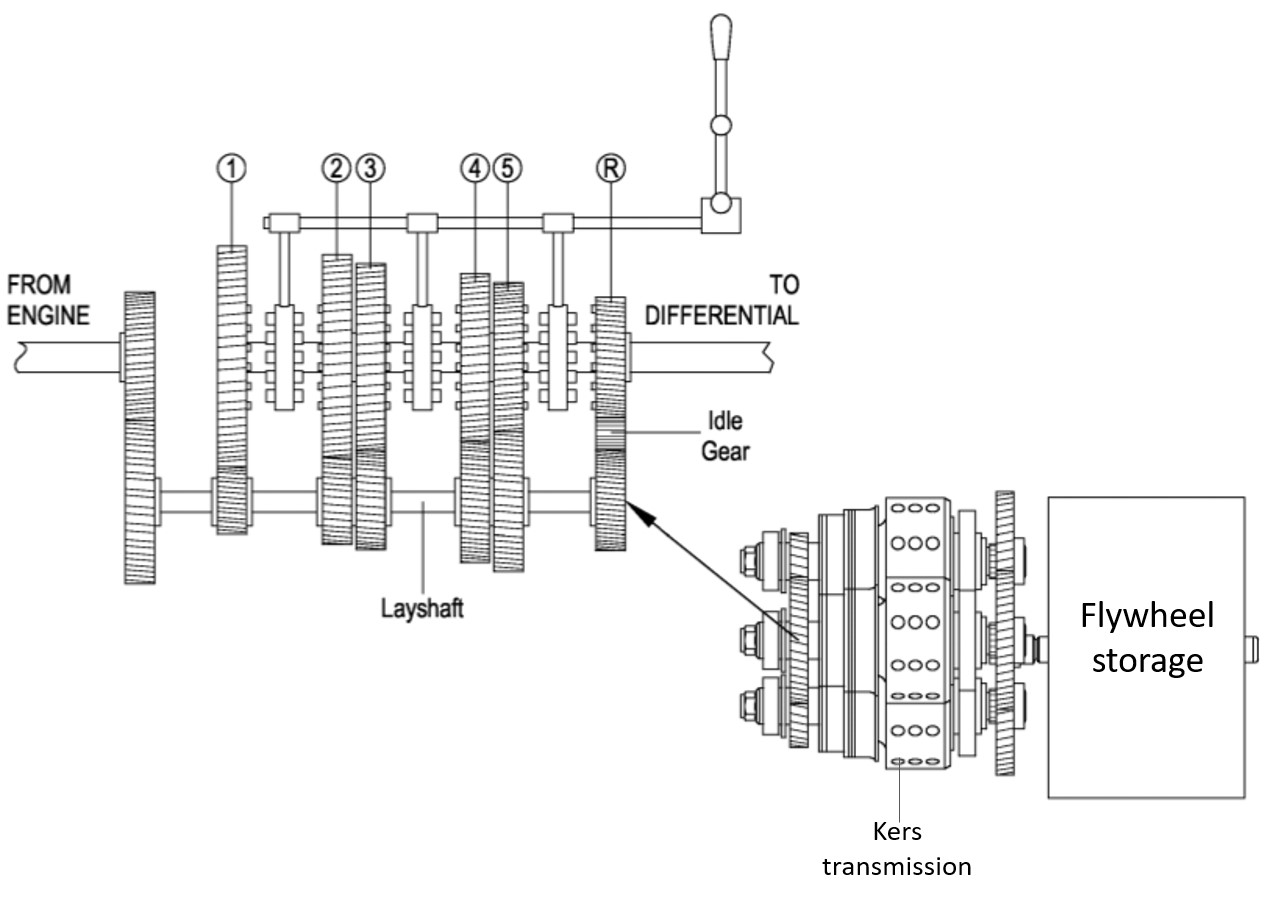
\includegraphics[width=.7\textwidth]{Images/State_of_the_art/Patent1}
\caption{Gearbox connection case}
\label{Patent1}
\end{figure}

Alternatively, the MKERS may be arranged to provide power to the car non-driving wheels (typically the rear ones). In this configuration (Fig.~\ref{Patent2}), the KERS transmission output is connected directly to the differential gear of the rear axle. This second configuration offers the advantage of treating the KERS as an optional, namely as a module that is completely separated from the driving wheels (the front ones in the present example) conventional powertrain.

\begin{figure}[H]
\centering
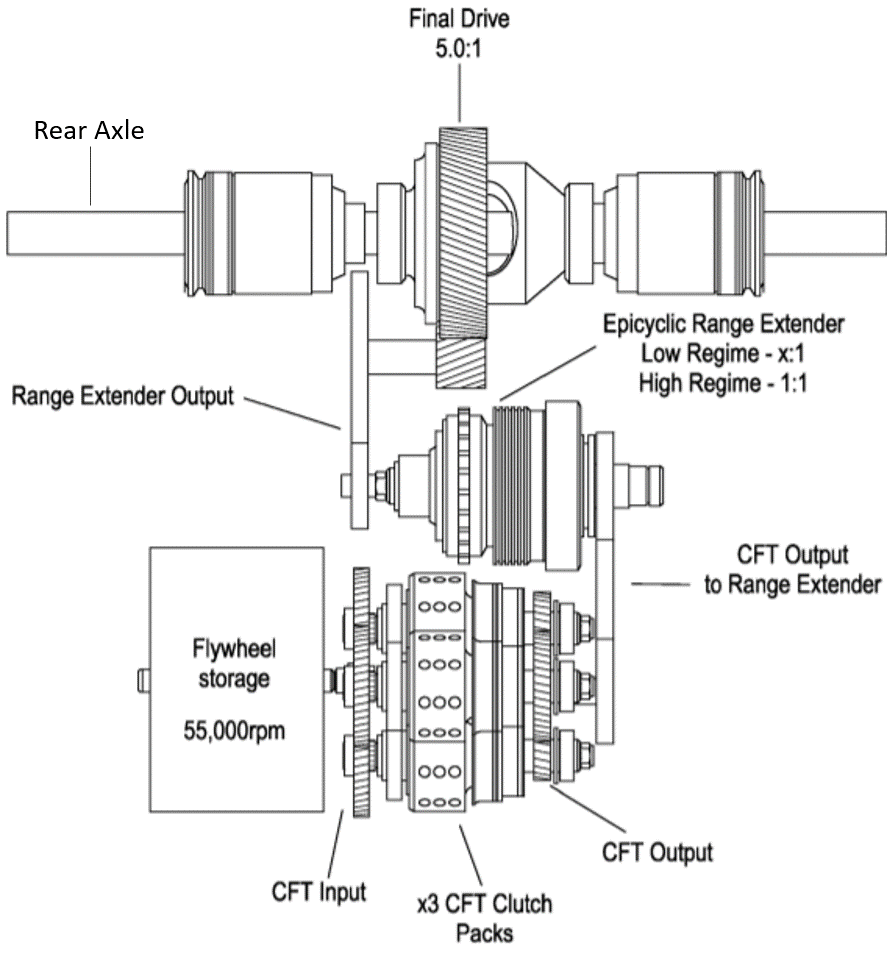
\includegraphics[width=.6\textwidth]{Images/State_of_the_art/Patent2}
\caption{Non-driving wheels connection case}
\label{Patent2}
\end{figure}

As above illustrated (Fig.~\ref{Patent2}), the MKERS transmission includes a cascade of two ratio sets connected in series: a clutched flywheel transmission (CFT) and a range extender. The CFT proposed in the invention includes three ratio sets arranged in series, each of which comprise two selectable ratios connected in parallel (“2x2x2” configuration). All ratios of each of the three ratio sets are selectable by friction clutches (Fig.~\ref{Patent3}). Moreover, all ratio sets include two clutches in such a way to have $2^{3}=8$ possible combinations of KERS ratios.

\begin{figure}[H]
\centering
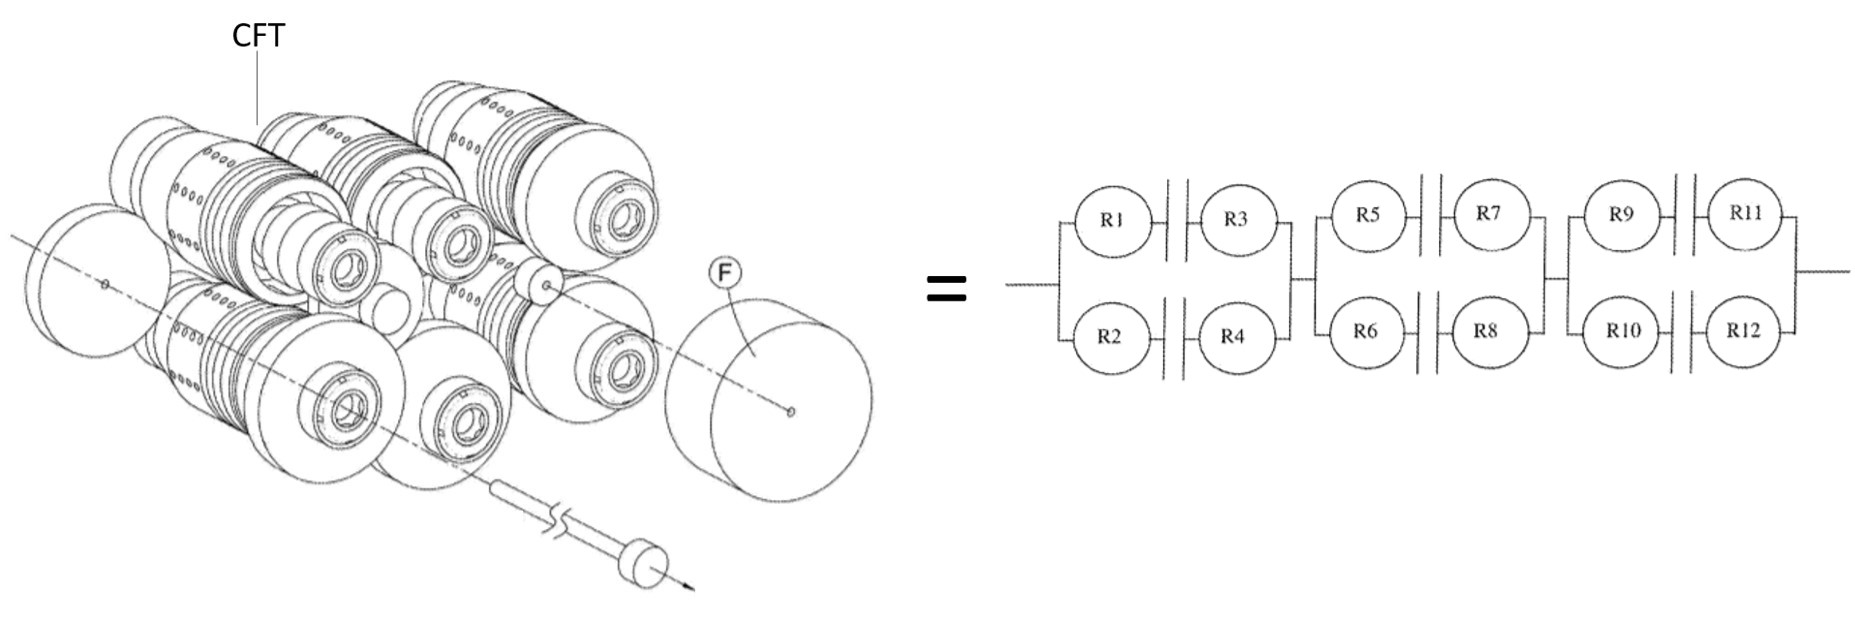
\includegraphics[width=.9\textwidth]{Images/State_of_the_art/Patent3}
\caption{CFT}
\label{Patent3}
\end{figure}

The CFT output is connected via transfer gears to a range extender (Fig.~\ref{Patent2}). This second component provides a second ratio set for increasing the number of MKERS selectable ratios. This second ratio set comprises a plurality of selectable ratios, each in parallel with one another. For example, an epicyclic gear train with two clutches would provide two selectable ratios. A range-extended CFT may offer marked performance enhancements over a non-range extended one in terms of efficiency of energy transfer from the wheels to the flywheel and back.  As shown in (Fig.~\ref{Patent1}), this second component may be excluded from the KERS transmission in the connection layout provided as first option. In fact, the number of available ratios to be exploited in the energy transfer process optimization is in this case already augmented by the ones provided by the conventional vehicle transmission (i.e. the gearbox).  An additional clutch may be as well included in the system to disconnect the MKERS from the vehicle powertrain under specific operating conditions.
As far as the numerical guidelines are concerned, the flywheel should be designed to have a storage capacity of 210 kJ and top rotational speeds of the order of 55.000 [rpm]. Moreover, the KERS transmission should be provided with a ratio spread (i.e. the maximum achievable ratio divided by the minimum one) of about 11, therefore outperforming the one offered by typical CVTs, which are usually characterized by a ratio spread ranging in the interval 4-7.  

\section{MKERS model}

The hybrid powertrain that has been considered in the present work is shown in fig.\ref{model}.   

\begin{figure}[H]
\centering
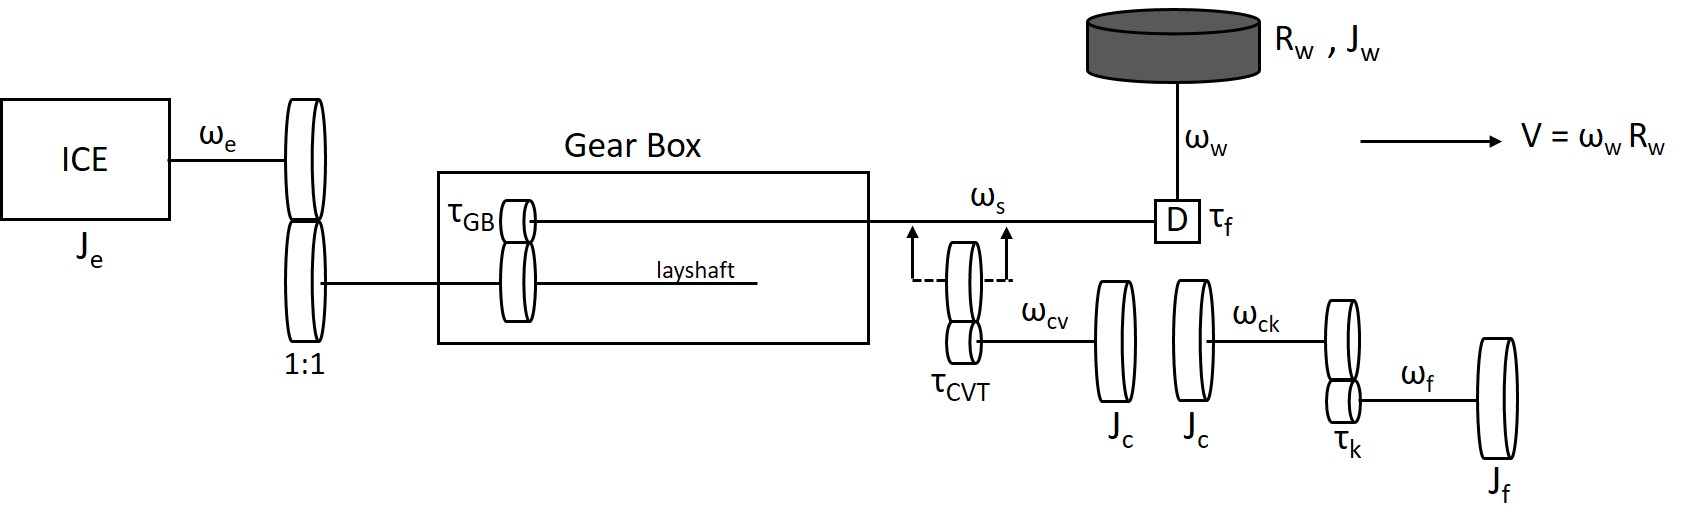
\includegraphics[width=1\textwidth]{Images/Model/Model.jpg}
\caption{Hybrid powertrain model}
\label{model}
\end{figure}

With respect to a standard powertrain, the proposed one is characterized by the presence of a high-speed flywheel, which is connected to the main driveline \textit{in parallel} with the prime mover (ICE). In particular, the flywheel powertrain uses a CVT (Torotrak\textsuperscript\textregistered\ model) for a smooth and fast charging and discharging of the flywheel and is as well provided with a 2x2x2 CFT device. The connection and disconnection operations of the flywheel from the system main driveline are carried out via a dedicated clutch. The model parameters that have been considered are the ones of a typical 2013 F1 car and are summarized in Tables 1 and 2.

\begin{table}[H]
\centering
\begin{tabular}{|c|c|}
 \hline 
 Parameter & Numerical Value\\ 
 \hline 
 $J_e$ &  $0.3\ [m^2*Kg]$\\   
 $J_w$ & $0.49\ [m^2*Kg]$ \\ 
 $R_w$ & $0.33\ [m]$ \\  
 $J_c$ & $0.1\ [m^2*Kg]$ \\ 
 $J_f$ & $0.026\ [m^2*Kg]$ \\  
 $M$ & $770\ [Kg]$ \\
 $\tau_f$ & $1/4.38$ \\
 $\tau_{cvt}$ & $0.4-2.5$ \\
 $\tau_k$ & $1/12-11/12$ \\  
 \hline 
\end{tabular} 
\label{params}
\caption{model parameters and variables}
\end{table}

\begin{table}[H]
\centering
\begin{tabular}{|c|c|}
 \hline 
 Transmission ratio & Numerical Value\\ 
 \hline 
 $\tau_1$ &  $1/3.08$\\  
 $\tau_2$ & $1/2.18$ \\ 
 $\tau_3$ & $1/1.63$ \\ 
 $\tau_4$ & $1/1.29$ \\  
 $\tau_5$ & $1/1.03$ \\ 
 $\tau_6$ & $1/0.84$ \\  
 $\tau_7$ & $1/0.69$ \\  
 \hline 
\end{tabular} 
\caption{Gearbox parameters }
\end{table}

In addition, four more simplifying assumptions have been considered. In particular, we assumed to have: 

\begin{itemize}
	\item Infinitely rigid suspensions;
	\item Lossless transmission (unitary transmission efficiency);
	\item Pure headway motion (zero slip coefficient);
	\item Instantaneous CVT ratio variation ($\dot{\tau}_{cvt}=\infty$).
\end{itemize}

This last assumption is justified by the fact that the time constants that characterize a typical CVT dynamic behaviour are of the order of $0.1$ [s] \cite{o}, whereas the overall energy transfer transient has a duration in the order of $1$ [s]. In this respect, the CVT ratio variation can be considered instantaneous at a first approximation.  
 
\newpage
 
\subsection{Equivalent model}

In order to focus on the KERS clutch engagement process, an equivalent model can be associated to the one of Fig.~\ref{model}. In particular, the aim of this kind of analysis is finding two equivalent inertias that are respectively reduced to the two shafts that are connected to the two different sides of the KERS clutch (Fig.~\ref{eq_model}).
From now on, we will address to these equivalent inertias as $J_{eq,v}$ and $J_{eq,k}$, where \textit{v} and \textit{k} stands respectively for vehicle and kers sides.
In other words, the target model can be represented as follows:

\begin{figure}[H]
\centering
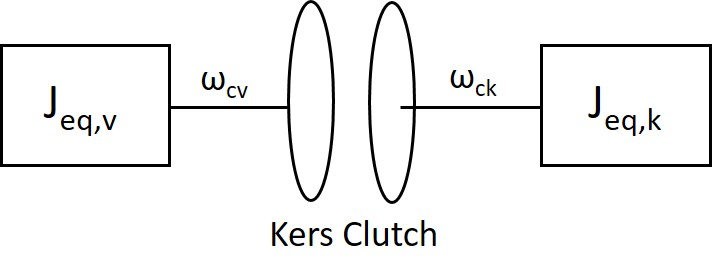
\includegraphics[width=0.6\textwidth]{Images/Model/Equivalent_model.jpg}
\caption{Hybrid powertrain equivalent model}
\label{eq_model}
\end{figure}

At this purpose, let us first of all consider all the kinematic constraints that characterize the original system:

\begin{eqnarray}
	\omega_{ck}&=&\tau_k \omega_f\\
	\omega_s &=&\tau_{cvt} \omega_{cv}\\
	\omega_w &=&\tau_f \omega_s\\
	\omega_s &=&\tau_{gb} \omega_e
\end{eqnarray}

These equalities yield

\begin{equation}
\omega_{cv}=\frac{\omega_w}{\tau_f*\tau_{cvt}} \Leftrightarrow \omega_{cv}=\frac{v}{\tau_f*\tau_{cvt}*R_w}\\
\end{equation}
\vspace{1mm}

The overall vehicle kinetic energy can be written as

\begin{align}
T_{vehicle}&=\frac{1}{2}Mv^2+\frac{1}{2}J_e\omega_e^2+ \frac{1}{2}(4J_w\omega_w^2)+\frac{1}{2}J_c\omega_{cv}^2 \\
	 &=\frac{1}{2}M(\tau_f\tau_{cvt}Rw)^2\omega_{cv}^2+\frac{1}{2}J_e\left(\frac{\tau_{cvt}}{\tau_{gb}}\right)^2\omega_{cv}^2+\frac{1}{2}\left[4J_w\left(\tau_f \tau_{cvt}\right)^2\right]\omega_{cv}^2+\frac{1}{2}J_c\ \omega_{cv}^2\\
	 &=\frac{1}{2}\left[M(\tau_f\tau_{cvt}Rw)^2+J_e\left(\frac{\tau_{cvt}}{\tau_{gb}}\right)^2+4J_w\left(\tau_f \tau_{cvt}\right)^2+J_c\right] \omega_{cv}^2\\
	 & \triangleq \frac{1}{2}J_{eq,v}\omega_{cv}^2 
\end{align}
\vspace{1mm}

The same kind of analysis can be performed on KERS side

\begin{eqnarray}
	T_{kers}&=&\frac{1}{2}J_c\omega_{ck}^2+\frac{1}{2}J_f\omega_f^2\\
	&=&\frac{1}{2}J_c\omega_{ck}^2+\frac{1}{2}\frac{J_f}{\tau_k^2}\omega_{ck}^2\\
	&=&\frac{1}{2}\left(J_c+\frac{J_f}{\tau_k^2}\right)\omega_{ck}^2\\
	&\triangleq & \frac{1}{2}J_{eq,k}\omega_{ck}^2
\end{eqnarray}

\section{Static analysis}

The complete energy transfer process consists of two main consecutive phases:

\begin{enumerate}
\item KERS clutch engagement process
\item KERS charge/discharge process
\end{enumerate}

At a first stage of the project, we have focused on the clutch engagement phase only by performing a static analysis of this process. In particular, with reference to the equivalent model derived in section 4.1, it is possible to model the KERS clutch engagement as an inelastic collision between the two rotating bodies $J_{eq,v}$ and $J_{eq,k}$. In this respect, if we denote by $\omega_c$ the clutch angular velocity after the collision, then we can apply as follows the angular momentum conservation law:

\begin{equation}
J_{eq,v}\omega_{cv}+J_{eq,k}\omega_{ck}=(J_{eq,v}+J_{eq,k})\omega_c\ \Rightarrow\ \omega_c= \frac{J_{eq,v}\omega_{cv}+J_{eq,k}\omega_{ck}}{J_{eq,v}+J_{eq,k}}\\
\end{equation}  

\subsection{KERS discharge}

Let us first of all focus on the KERS discharge process, which takes place during a vehicle acceleration event. For the sake of simplicity, suppose that the initial vehicle velocity $v_0$ is zero (i.e. the vehicle is initially at standstill). The variation of the vehicle kinetic energy due to the clutch engagement can be calculated as

\begin{eqnarray}
	\Delta E_{vehicle}&=&\frac{1}{2}Mv_f^2-\frac{1}{2}Mv_0^2\\
	                  &=&\frac{1}{2}M(\tau_f \tau_{cvt}Rw)^2\omega_c^2-\frac{1}							  {2}Mv_0^2\\
	                  &=&\frac{1}{2}M\left(\frac{J_{eq,v}\omega_{cv}+J_{eq,k}       					  \omega_{ck}}{J_{eq,v}+J_{eq,k}}\right)^2(\tau_f \tau_{cvt}						  Rw)^2-\frac{1}{2}Mv_0^2
\end{eqnarray}  

Letting $v_0=0$, we get

\begin{eqnarray}
\Delta E_{vehicle}&=&\frac{1}{2}M\left(\frac{J_{eq,k}}{J_{eq,v}+J_{eq,k}}								 \right)^2(\tau_f \tau_{cvt}Rw)^2\omega_{ck}^2\\
                  &=&\frac{T_{0,k}}{J_f}M\left(\frac{J_{eq,k}}{J_{eq,v}+J_{eq,k}}					     \right)^2(\tau_f \tau_{cvt}Rw)^2 \tau_k^2
\label{energy_vehicle}
\end{eqnarray}
where

\begin{equation}
T_{0,k} = \frac{1}{2}J_f\omega_{f,0}^2
\end{equation}

Under the aforementioned assumptions, the vehicle kinetic energy variation can be therefore simply written as a linear function of the KERS initial kinetic energy. Once the vehicle energy profiles have been computed (Fig.\ref{en_comp_acc}), the vehicle velocity profiles can be as well derived by exploiting the following equation
\begin{equation}
\Delta v_{vehicle} = v_f = \sqrt{\frac{2\Delta E_{vehicle}}{M}}
\end{equation}

\begin{figure}[H]
\captionsetup{font=small, justification=centering}
\centering
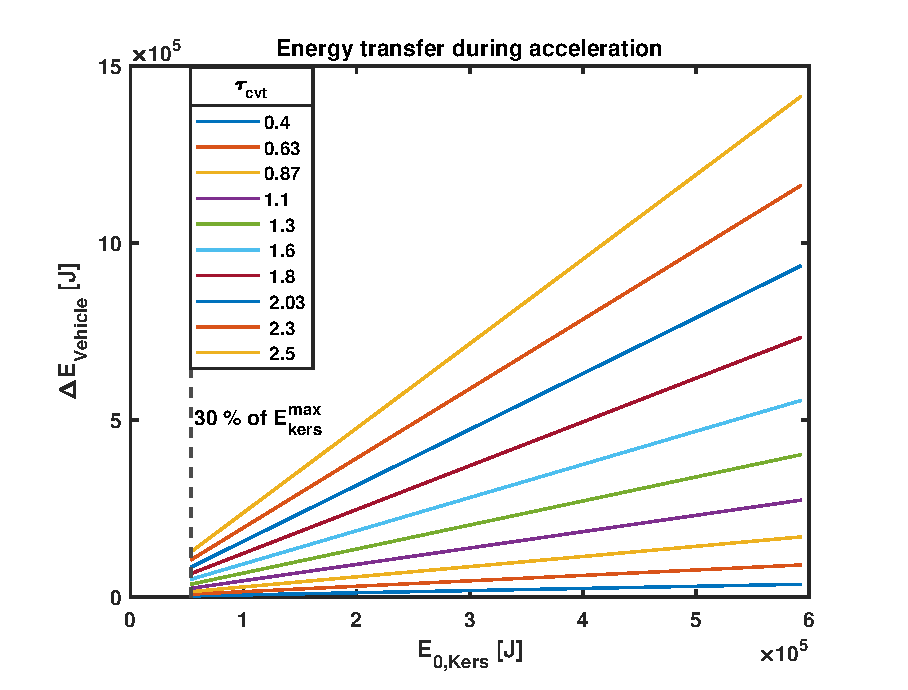
\includegraphics[width=.49\textwidth]{Images/Results_new/Univariate_SteadyState/en_comp_acc.eps}\hfill
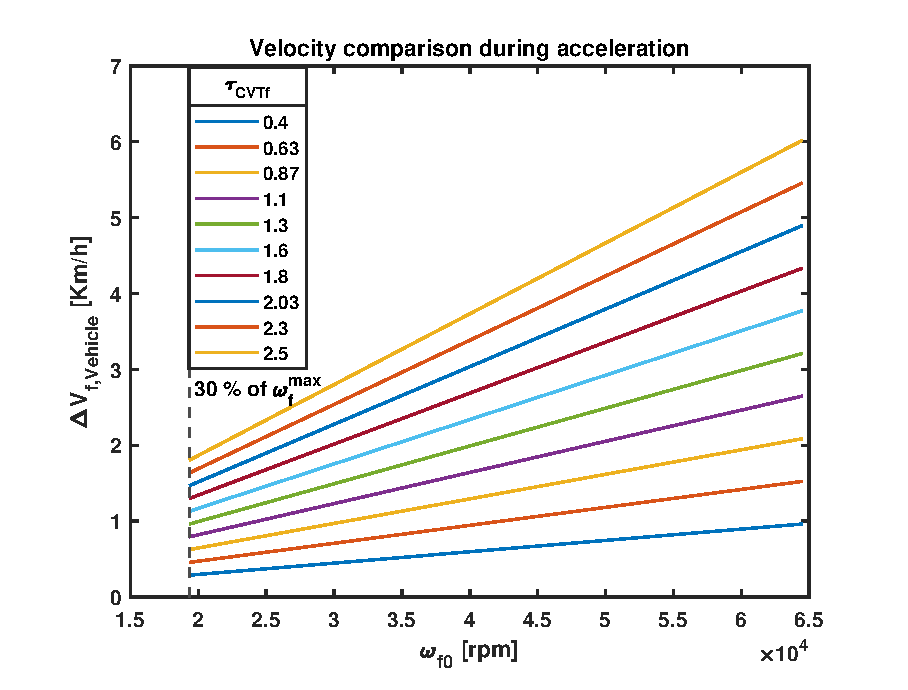
\includegraphics[width=.49\textwidth]{Images/Results_new/Univariate_SteadyState/vel_comp_acc.eps}
\caption{Energy (left) and velocity (right) gained by the vehicle thanks to the kers' clutch engagement}
\label{en_comp_acc}
\end{figure}

In particular, the above profiles have been calculated by plugging into \eqref{energy_vehicle} the values of the KERS initial energy for all the possible initial flywheel angular velocities in the interval $[0.3 \, \omega_f^{max}, \omega_f^{max}]$, where the maximum admissible value for the flywheel angular velocity has been set to $\omega_f^{max}=64500$ [rpm]. This value is in general upper-limited by the characteristics of the material that the flywheel is made of. In fact, increasing the flywheel velocity beyond the critical stress levels that material can withstand could result in flywheel damage and destruction.

Furthermore, the curves are parameterized with respect to $\tau_{cvt,f}$. In other words, we assumed that, at the beginning of the process, $\tau_{cvt,0} = \tau_{min} = 0.4$ and we also assumed that $\tau_{cvt}$ is let free to evolve during the engagement process up to its maximum admissible value $\tau_{cvt,f} = \tau_{max} = 2.5$. In this respect, all the quantities \textit{before} the collision are calculated with respect to $\tau_{cvt,0}$ and all the quantities \textit{after} the collision are parameterized with respect to $\tau_{cvt,f}$.\\ However, the only really feasible choice is to keep $\tau_{cvt,f} = \tau_{cvt,0} = \tau_{min}$ during the whole engagement transient. In fact, the aim of the clutch engagement process is in this case to dissipate a certain amount of the KERS kinetic energy in such a way to \textit{enter} the CVT admissibility range. In other words, the flywheel speed has to be reduced (and the vehicle one has to be increased) in such a way that 

\begin{equation}
\tau_{min} < \tau_{cvt} \left(= \frac{\omega_w}{\omega_f \tau_f \tau_k}\right) < \tau_{max}
\label{range_tau_cvt}
\end{equation}
          
Once this condition is met, the clutch can be considered as completely engaged (i.e. the slipping between the clutch disks is zero) and the second phase of the energy transfer process can take place: the $\tau_{cvt}$ is now let free to change and opposite angular accelerations of the vehicle wheel and flywheel are established, which allows the mechanical energy transfer between the two components to take place. In other words, the $\tau_{cvt}$ parameter plays the role of a feedback control action, whose expression~\eqref{range_tau_cvt} is univocally determined by the systems kinematic constraints, and whose value is saturated between $\tau_{min}$ and $\tau_{max}$. The clutch slipping transient allows the system to \textit{escape} the saturation limits of this component. This operation is fundamental in such a way to allow the energy transfer process to continue also after the clutch full engagement, which is indeed only possible with a time-varying transmission ratio between wheels (sink) and flywheel (source). For these reasons, the only curve of Fig. \ref{en_comp_acc} we should make reference to is the one parametrized in $\tau_{cvt}=0.4$. This shows that, during the clutch engagement process only, the vehicle can gain an average speed of about $25$ [Km/h].\\For completeness, the same analysis has been repeated by considering the energy transfer also as a function of each of the eight selectable ratios $\tau_k$ of the 2x2x2 CFT. In particular, in Fig. \ref{en_comp_acc_3D} the results obtained for $\omega_{f,0} = \omega_f^{max}$ are reported. 

\begin{figure}[H]
\captionsetup{font=small, justification=centering}
\centering
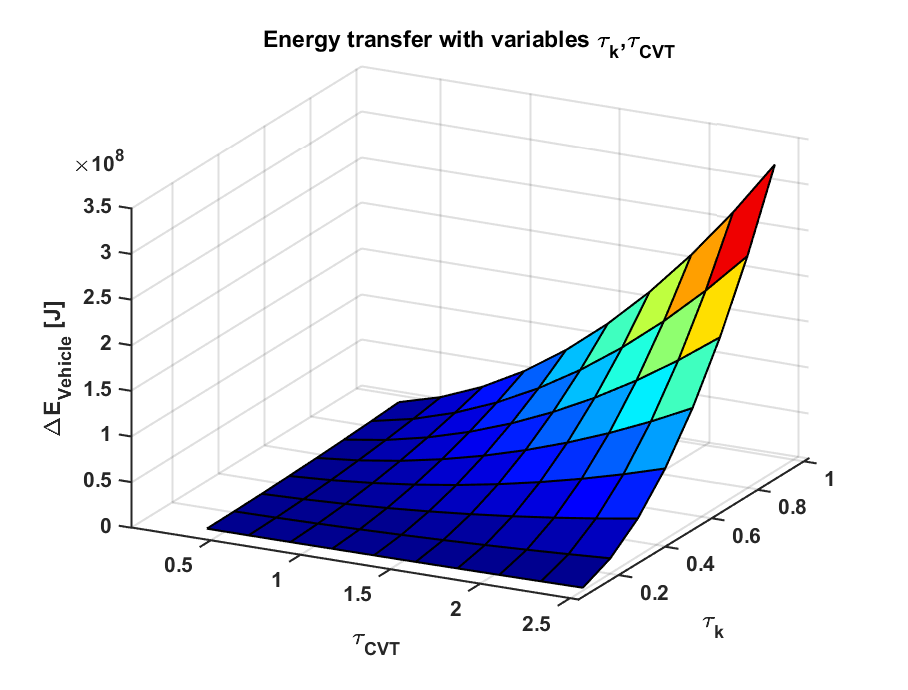
\includegraphics[width=.55\textwidth]{Images/Results_new/Univariate_SteadyState/en_comp_acc_3D.eps}
\caption{Energy gained by the vehicle thanks to the kers' clutch engagement}
\label{en_comp_acc_3D}
\end{figure}    

This kind of bivariate analysis shows that the most convenient choice for $\tau_k$ is in this case $\tau_{k,max}$. Note that, differently from $\tau_{cvt}$, $\tau_k$ remains fixed during the whole energy transfer process.

\subsection{KERS charge}

A similar study can be performed in the opposite situation, to which we have been referring as \textit{regenerative braking}. Supposing now that $\omega_{f,0}=0$ [rpm], we get

\begin{eqnarray}
\Delta E_{kers}&=&\frac{1}{2}J_f\omega_{f,f}^2\\
               &=&\frac{1}{2}J_f\frac{\omega_{c}^2}{\tau_k^2}\\
               &=&\frac{1}{2}J_f\left(\frac{J_{eq,v}}{J_{eq,v}+J_{eq,k}}					          \right)^2\frac{\omega_{cv}^2}{\tau_k^2}\\               
               &=&\frac{T_{0,v}}{M}J_f\left(\frac{J_{eq,v}}{J_{eq,v}+J_{eq,k}}					     \right)^2\left(\frac{1}{\tau_f \tau_{cvt}Rw}\right)^2\frac{1}    						 {\tau_k^2} 
\end{eqnarray}
where
\begin{equation}
T_{0,v} = \frac{1}{2}Mv_0^2.
\end{equation} 

Once again the KERS speed variation can be calculated as 

\begin{equation}
\Delta \omega_{kers} = \omega f,f = \sqrt{\frac{2\Delta E_{kers}}{J_f}}
\end{equation}

\begin{figure}[H]
\captionsetup{font=small, justification=centering}
\centering
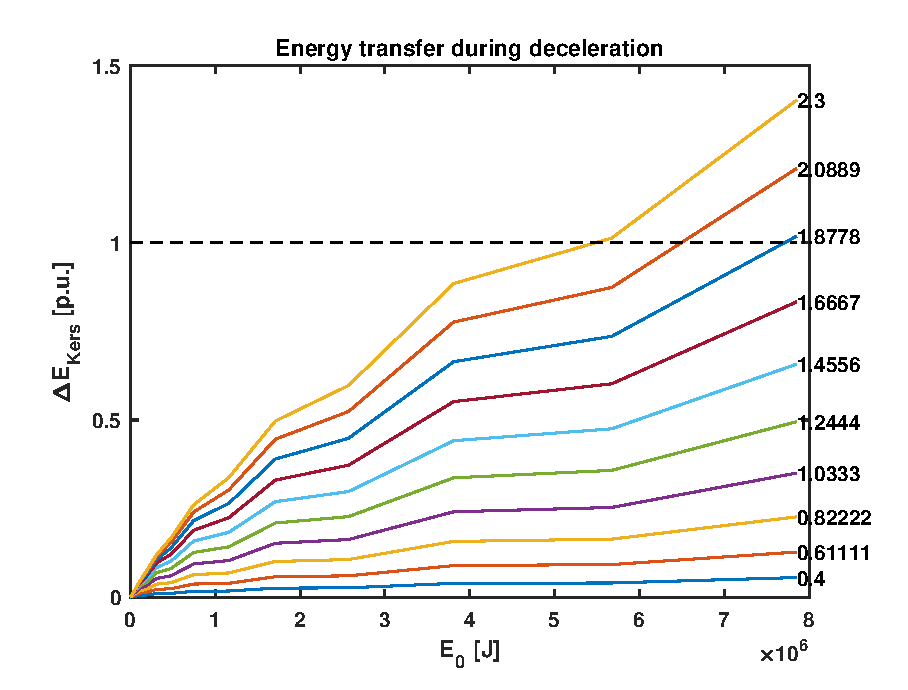
\includegraphics[width=.49\textwidth]{Images/Results_new/Univariate_SteadyState/en_comp_dec.eps}\hfill
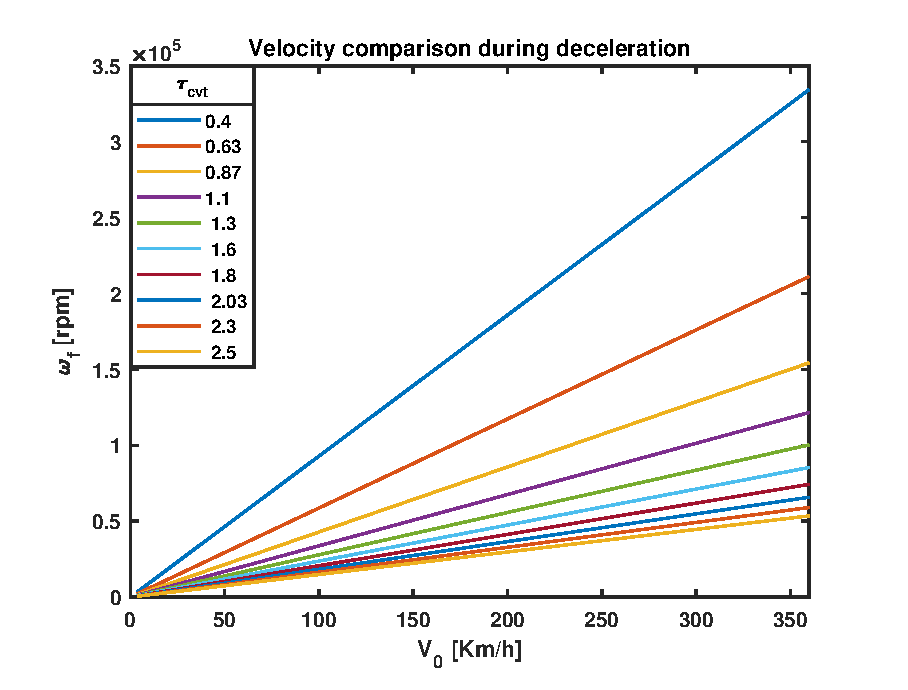
\includegraphics[width=.49\textwidth]{Images/Results_new/Univariate_SteadyState/vel_comp_dec.eps}
\caption{Energy (left) and velocity (right) gained by the kers thanks to the kers' clutch engagement}
\label{en_comp_dec}
\end{figure}

The energy and velocity curves are this time computed considering all possible initial vehicle speeds in the range $[0, 360]$ [Km/h]. For the same reasons above explained, the clutch engagement process should be this time carried out keeping $\tau_{cvt}$ constant at its maximum value $\tau_{cvt,max}$. In fact, the clutch slip will allow in this case to dissipate some of the initial vehicle kinetic energy until the Torotrak saturation limit (i.e. $\tau_{cvt,max}$) is overcome and the second phase of the energy transfer process can take place.\\As a consequence, the curve of Fig. \ref{en_comp_dec} we make reference to is the one parametrized by $\tau_{cvt}=2.5$. This shows that, during the clutch engagement process only, the kers can be re-charged up to the 70\% of its full charge.   
A similar bivariate analysis to the one provided for the discharge process has been in this case as well performed:

\begin{figure}[H]
\captionsetup{font=small, justification=centering}
\centering
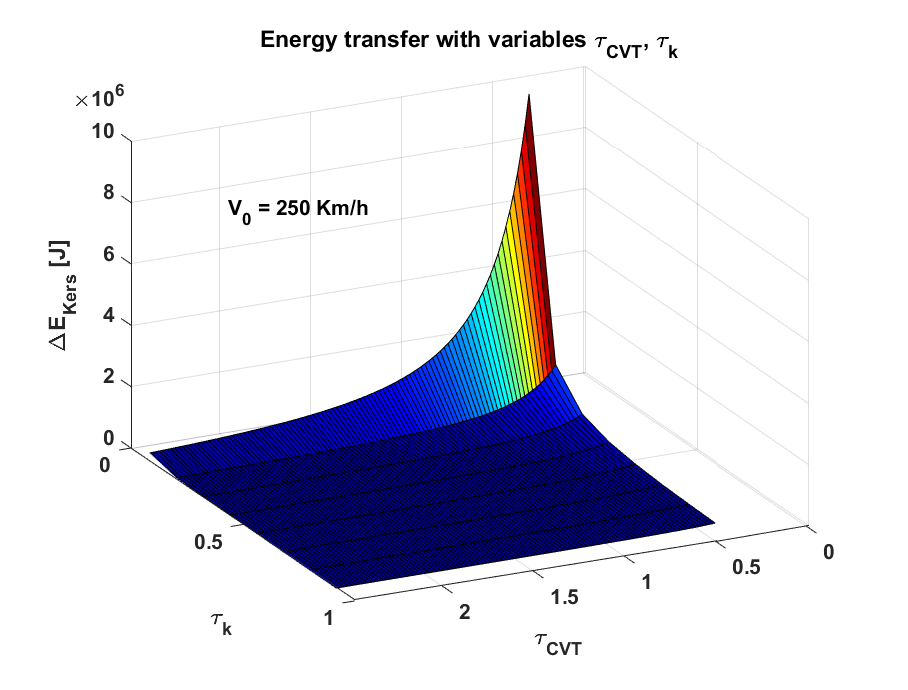
\includegraphics[width=.7\textwidth]{Images/Results_new/Univariate_SteadyState/en_comp_dec_3D.eps}
\caption{Energy gained by the kers thanks to the kers' clutch engagement}
\label{en_comp_dec_3D}
\end{figure}  

The obtained profiles show that the best-performing choice for the 2x2x2 CFT ratio during the KERS re-charge  is $\tau_k=\tau_{k,min}$.

\section{Dynamic analysis}

In order to understand in a proper way the dynamics of the regenerative braking, the lagrangian approach has been taken. It has many advantages with respect to the Newton laws formulation, because it relies on the definition of generalized coordinates and on the expression of the total energy of the system which is evolving in time. 

This aspect fits perfectly in the case of a KERS system, because the system is characterized just by the kinetic energy of the flywheel and the wheels. No potential field must be introduced, since it is assumed that the vehicle is traveling on a flat road (as it happens in F1 races).

\subsection{Lagrangian mechanics}

The lagrangian mechanics is an analytic way of describing the motion of a mechanical system using the results of calculus of variation. 

First of all, one defines a set of generalized coordinates $\bm{q} = [q_1, q_2, \dots, q_N]$ and the derivative $\dot{\bm{q}}$. These two variables describe in a unique way the motion of the system. The second step is to define the so--called Lagrangian
\begin{equation}
L(\bm{q},\dot{\bm{q}}) = T(\bm{q},\dot{\bm{q}}) - U(\bm{q})
\label{lagrangian}
\end{equation}
where $T(\cdot)$ represents the kinetic energy of the system, and $U(\cdot)$ indicates the potential energy.

In order to pass from the function $L$ to the equation of motion, one has to minimize the so called action, which is a functional of the following shape
\begin{equation}
S = \int_{t_1}^{t_2} L(\bm{q},\dot{\bm{q}}) \, dt
\label{action_functional}
\end{equation}
where $t_1, t_2$ are the instants at which the evolution starts and ends, respectively.

A general result in physics states that, in general, in a conservative field a particle will travel its path minimizing the action. This means that the dynamics of a certain system subject only to conservative forces respect the minimum action principle. From a mathematical point of view, it corresponds to find the minimum of the functional $S$, that is
\begin{equation}
dS = 0.
\label{minimum_action}
\end{equation}

Due to the definition of $S$, the~\eqref{minimum_action} is equivalent to write
\[
dS = \int_{t_1}^{t_2} \Biggl( \dfrac{\partial L}{\partial \bm{q}}d\bm{q} + \dfrac{\partial L}{\partial \dot{\bm{q}}}d\dot{\bm{q}}\Biggr) \, dt.
\]

After applying integration by parts, the problem reduces to solving the Euler--Lagrange equations, i.e.
\begin{equation}
\dfrac{d}{dt} \dfrac{\partial L}{\partial \dot{\bm{q}}} - \dfrac{\partial L}{\partial \bm{q}} = 0.
\label{euler_lagrange}
\end{equation}

Once having computed these equations\footnote{The number of Euler--Lagrange equations is exactly equal to the dimension of $\bm{q}$, i.e. each generalized coordinate is characterized by its own dynamics and it will evolve according to the conservative forces to which it is subject to.} one gets the dynamics of the system subject to the conservative forces. Since this approach does not take into account other contributions coming from non--conservative fields (friction, dissipations, external inputs or disturbances) it is necessary to introduce these elements (if any) directly as forces or torques. Note that modeling these quantities can be very difficult from a physical point of view and in many cases requires a lot of experiments, ending up sometimes with very complicated mathematical expressions.

Depending on the nature of the physical system, the lagrangian mechanics will formulate torque equations for rotational elements (like a flywheel) and force equations for translational elements (like a mass changing its position in the space).

\subsection{KERS dynamics}

Using the lagrangian mechanics, the mathematical model of a KERS system has been built. This model needs to take into account the motion of the flywheel and the vehicle itself. Having this in mind, a straightforward choice is to pick $\omega_f$ and $\omega_w$ as generalized coordinates. Indeed, the system can be fully described using these two quantities, since the angular velocities of the other components can be obtained starting from the aforementioned two with some manipulations involving the transmission ratios and the efficiency. 

Under the hypothesis of flat road, the whole system does not have mechanical potential energy. So the lagrangian is given by the two kinetic energy contributions:
\begin{equation}
L = T_{\textup{vehicle}} + T_{\textup{flywheel}} = \dfrac{1}{2}J_{eq}\omega_w^2 + \dfrac{1}{2}J_f\omega_f^2. 
\label{lagrangian_kers}
\end{equation}

As already explained, this particular lagrangian will result into two torque equations which will describe the dynamics of the KERS system.

Applying~\eqref{euler_lagrange} to~\eqref{lagrangian_kers}, one gets the two equations
\begin{equation}
\begin{split}
J_{eq}\, \dot{\omega}_w & = 0 \\
J_f\, \dot{\omega}_f & = 0.
\end{split}
\label{free_dynamics}
\end{equation}

Now it is necessary to introduce the non--conservative torques, which will complete the dynamics of the regenerative braking. To do this, it is needed to split the model according to the phase in which the KERS is used.

\subsubsection{KERS charge}

In the charge phase, the KERS brakes the vehicle, which is traveling at a certain speed $v_0$. This means that the clutch engages the flywheel which will absorb the kinetic energy lost by the vehicle by changing the transmission ratio of the Torotrak, which from now on will be denoted simply as $\tau$. Since $\tau = \dfrac{\omega_w}{\omega_f \tau_f \tau_k}$, during the charge $\tau$ will decrease and at the very beginning of the process will be saturated at his maximum value $\tau_{max}$, since the difference between the two angular velocities is too big, especially when the flywheel is at rest ($\omega_f = 0$ [rpm]). During the amount of time in which $\tau = \tau_{max}$ the clutch engages the flywheel with slipping: the clutch engagement can be exploited to reduce the transient of the charge by using an active element (actuator) which should be able to vary the normal force $F_N$ exerted on the clutch plates. The flywheel will be ruled out when it reaches the maximum velocity or when $\tau = \tau_{min}$, i.e. the CVT is not able to transfer the energy from the vehicle to the flywheel.

Having in mind the physics of the system, the non--conservative contributions to be included are:
\begin{itemize}
\item the braking torque $T_b$. It is assumed that the braking action is abrupt, and so it is computed as the weight unloaded on the wheels (a constant signal acting during the whole dynamics)
\begin{equation}
T_b = - 0.9 M g R_w; 
\label{braking_torque}
\end{equation}
    
\item the clutch engagement slipping torque $T_{cl}$. It contributes to the dynamics only when $\tau = \tau_{max}$: afterwards, it is zeroed since the clutch is completely engaged. It can be expressed as a function of the normal force applied to the plates in the following way \cite{clutch}
\begin{equation}
T_{cl} = kF_N \textup{sgn} (\omega_{cv} - \omega_{ck})
\label{clutch_torque}
\end{equation}
where $k = \frac{4}{3}R_{cl} \mu_d$ is the equivalent clutch radius, $\mu_d$ is the dynamic friction coefficient, $R_{cl}$ is the radius of the clutch plates, and, as already said, $F_N$ is the normal force applied to the clutch plates, which in the case of passive process, is a constant fixed by the manufacturer;
\item the aerodynamic torque which decelerates the vehicle $T_{aero}$. It has a standard expression and it depends on the air density $\rho$, the surface exposed $S_f$ and the drag coefficient $C_x$:
\begin{equation}
T_{aero} = \dfrac{1}{2}\rho C_x S_f \omega_w^2 R_w^3 = d\omega_w^2.
\label{aero_torque}
\end{equation}
\end{itemize}

In this dissertation, the rolling resistance has been neglected for the sake of simplicity.

Taking into account these contributions, and defining $\tau_{t} = \dfrac{1}{\tau_f \tau_k}$ the~\eqref{free_dynamics} is transformed into 
\begin{equation}
\begin{split}
J_{eq\,} \dot{\omega}_w & = T_b - T_{aero} - \dfrac{T_{cl}}{\tau \tau_f} \\
J_f\, \dot{\omega}_f & = -\dfrac{\tau}{\tau_{t}} T_b + T_{cl} \tau_k
\end{split}
\label{kers_full_dynamics_charge}
\end{equation}

It is worth noting that, due to the presence of $T_{aero}$ and $T_{cl}$, this is a nonlinear driftless system of the form
\[
\dot{x} = g(x)u + p(x)w 
\]
where $g(x) = k \, \textup{sgn} (\omega_{cv} - \omega_{ck}) [-\frac{1}{\tau \tau_f} , \tau_k]^T$, $u = F_N$ (control action), $p(x) =\left[  \begin{smallmatrix}
1 & -\omega_w^2 \\
-\frac{\tau}{\tau_t} & 0
\end{smallmatrix}\right] $
and $w = [T_b, d]^T$. Note that, due to the definition of $\tau$, it can be considered a forced saturated control, whose variation realizes the passage of energy from the vehicle to the flywheel. It follows that $\tau$ is not a free user--defined signal, but it is a state--dependent control obliged to be
\[
\tau = \dfrac{\omega_w}{\omega_f} \tau_t.
\]

\subsubsection{KERS Discharge}

The next step is modeling the discharge phase. In this scenario, the flywheel is supposed to be fully charged ($\omega_f = \omega_f^{max}$) and the driver, through a button on the steering wheel, triggers the KERS, causing the passage of energy from the flywheel to the vehicle wheels. During the discharge of the flywheel, $\tau$ is increasing (symmetric with respect to the charge phase, as expected). As before, during the whole period in which $\tau = \tau_{min}$ the clutch is in the slipping condition and $\tau$ does not vary until the clutch engagement is completed. Again, an engagement control can be performed, decreasing the discharge transient and increasing the vehicle acceleration in a short period.

Eventually, as also suggested in the patent which has been taken as a reference, the flywheel will be ruled out when it reaches the 30\% of its maximum charge\footnote{This is convenient for two reason. Firstly, many full charges and discharges of the flywheel during a race will deteriorate the component which has, in any case, a high cost. Secondly, excluding the KERS when $\omega_f = 0.3\,\omega_f^{max}$ allows a more efficient and rapid charge in the next phase.} or when $\tau = \tau_{max}$.

Having in mind the physics of the system, the main non--conservative contributions to be added are:

\begin{itemize}
\item accelerating torque $T_a$. It is a constant signal that represents the torque that the KERS gives to the vehicle. It is given by the following expression
\begin{equation}
T_a = M_{K} g R_w
\label{accelerating_torque}
\end{equation}
where $M_K$ is the mass of the whole KERS system, including not only the flywheel but also the mass of the other components (Torotrak, transmission lines, ...);
\item aerodynamic torque $T_{aero}$. Same as charge case (see~\eqref{aero_torque});
\item clutch engagement torque $T_{cl}$. Same as charge case (see~\eqref{clutch_torque}), but with inverted signs (in this scenario, the energy transfer happens in the opposite direction through the same clutch);
\item engine torque $T_e$. During the discharge case, of course, the vehicle keeps using the engine, which is ruled out during the charge case. It means that the torque exerted by the KERS system is added to the one provided by the engine\footnote{The engine continues working during the KERS discharge. The contribution of the KERS is providing more torque, increasing the wheels angular velocity which in the most common scenario could be saturated at the maximum velocity that the vehicle can reach thanks to the engine characteristics (about 315 [km/h])}, so increasing the vehicle maximum velocity. 

The engine torque depends on many different parameters, but in general it can be considered as a function of the engine crankshaft angular velocity $\omega_e$. Usually, the manufacturer provides the engine curve from which one can derive a polynomial law through curve fitting. The easiest choice is to approximate the torque curve with a second degree polynomial. In this work, the torque has been fitted starting from the curves available, related to F1 engines. The expression of the engine torque is the following
\begin{equation}
T_e = a_0 + a_1\,\omega_e + a_2 \, \omega_e^2 = 88.5 + 1.4 \,\omega_e -8.36 \times 10^{-4}\,\omega_e^2.
\label{engine_torque}
\end{equation}

Note that, in general, when using a second degree polynomial fitting, the coefficient $a_2$ must be negative, because the torque curve concavity is facing down.  
\end{itemize}

Also in this case, the rolling resistance has been neglected.

Taking into account these contributions, and defining again $\tau_{t} = \dfrac{1}{\tau_f \tau_k}$ the~\eqref{free_dynamics} is transformed into 
\begin{equation}
\begin{split}
J_{eq}\, \dot{\omega}_w & = T_a + T_e - T_{aero} + \dfrac{T_{cl}}{\tau \tau_f}  \\
J_f\, \dot{\omega}_f & = -\dfrac{\tau}{\tau_{t}} T_a - T_{cl} \tau_k
\end{split}
\label{kers_full_dynamics_discharge}
\end{equation}

This second model results into a nonlinear system\footnote{Note that the system is no more driftless, as it happens for the one used in the charge case, since the engine torque depends directly from the state variables $\omega_w$.} of the form
\[
\dot{x} = f(x) + g(x)u + p(x)w 
\]
where $f(x) = [T_e(\omega_w), 0]^T$, $g(x) = k \, \textup{sgn} (\omega_{cv} - \omega_{ck}) [\frac{1}{\tau \tau_f} , -\tau_k]^T$, $u = F_N$ (control action), $p(x) =\left[  \begin{smallmatrix}
1 & -\omega_w^2 \\
-\frac{\tau}{\tau_t} & 0
\end{smallmatrix}\right] $
and $w = [T_a, d]^T$. Note that $T_e(\cdot)$ can be written as a function of $\omega_w$ taking into account the driveline relation between the crankshaft and the wheels angular velocities, i.e.
\begin{equation}
\omega_w = \tau_{\textup{GB}} \tau_f \omega_e
\label{driveline_relation}
\end{equation}
where $\tau_{\textup{GB}}$ is one of the seven ratios which will depend on the gear inserted during the acceleration phase.

\section{Simulation and Results}

In this section various simulations for both cases will be presented so validating the proposed dynamics. Moreover some results in the case a constant force is applied to the cluch plates will be shown and this will be compared with a PID control approach.
\subsection{KERS charge}

For this scenario the initial velocity of the vehicle has been chosen as $v_0 = 300$ km/h and the F1 car is in the proximity of a curve. The control law which has been applied is a PID with only a proportional gain. In particular $K_p = 50$. In Fig.~\ref{fig: Engagement_plus_KERS_Vel_Charge} it is shown how the engagement process works. When the Torotrak ratio $\tau$ is saturated, the two angular velocities $\omega_{c,v}$ and $\omega_{c,k}$ have their own independent behavior. Then at about $0.6$ seconds the clutch engages the flywheel, so the two angular velocities are constrained to have the same behavior. This is maintained until the transmission ratio, which is decreasing in time, reaches its minimum value. 

Note also that during the interval in which the angular velocities are constant, there is a linear behavior for the $\tau$, which is consistent with its definition. On the KERS side, the full charge happens in $1.2$ seconds. After the charge is complete the value of the angular velocities $\omega_{c,v}$ and $\omega_{c,k}$ remains the same because the energy which is exchanged between the vehicle and the flywheel remains constant\footnote{This actually means that when $\omega_f = \omega_f^{max}$ the Torotrak ratio $\tau$ does not have reached its minimum value yet.}. The behavior of the $\tau$ is shown in Fig.\,\ref{fig: CVT_ratio_charge}.

\begin{figure}[H]
\centering
\subfloat[][\emph{} \label{fig: ClutchEng}]
{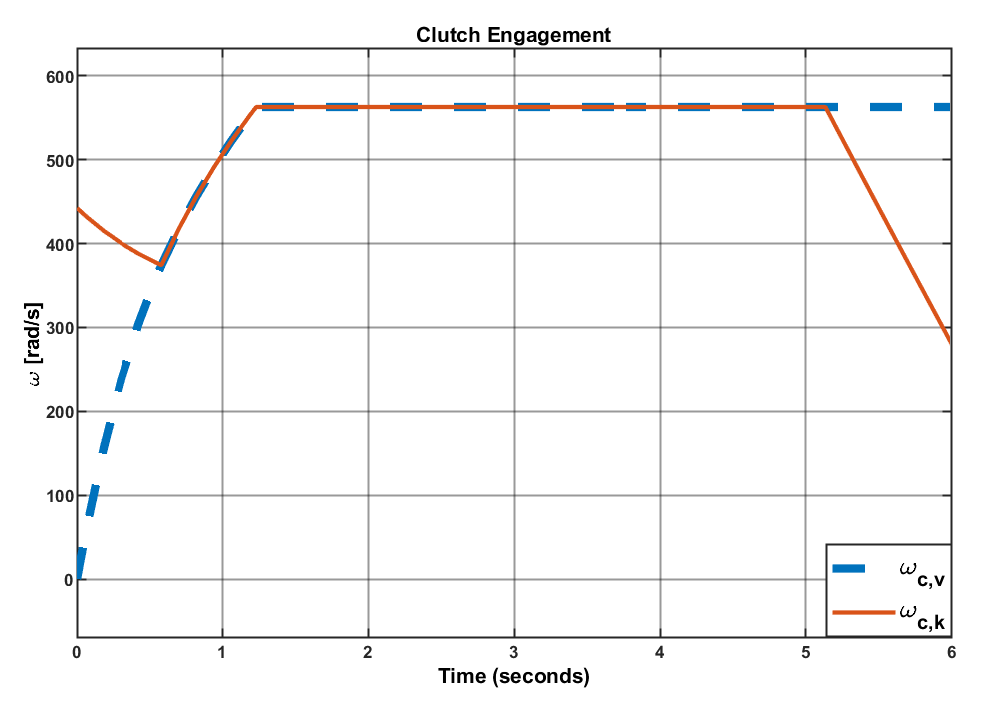
\includegraphics[width=.45\textwidth]{Images/Results_Dynamics/Charge/Clutch.eps}} \quad
\subfloat[][\emph{} \label{fig: ClutchVel}]
{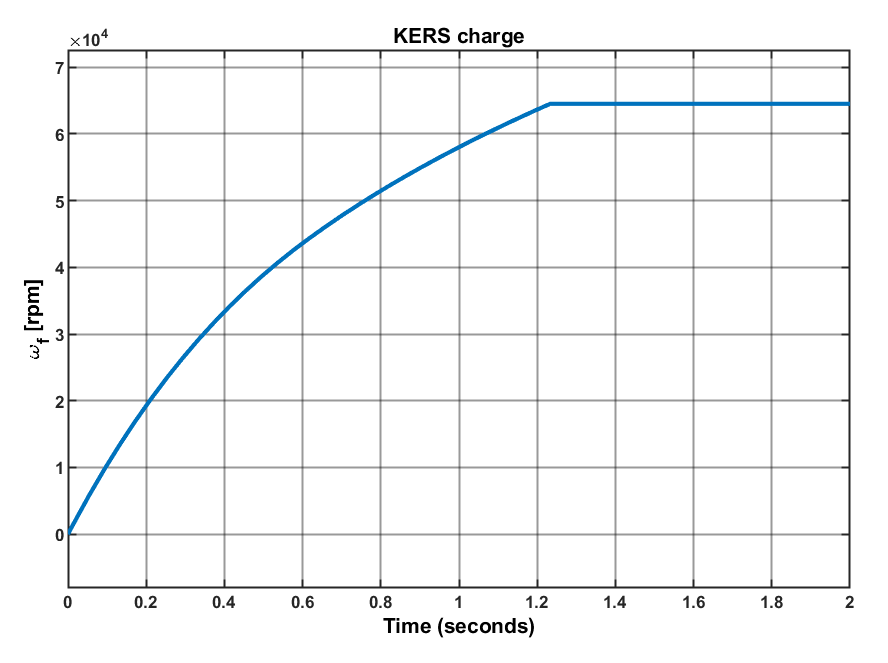
\includegraphics[width=.44\textwidth]{Images/Results_Dynamics/Charge/KERS_Vel.eps}} \\
\caption{Comparison between Clutch Engagement \protect\subref{fig: ClutchEng} and KERS angular velocity \protect\subref{fig: ClutchVel}}
\label{fig: Engagement_plus_KERS_Vel_Charge}
\end{figure}

\begin{figure}[H]
\centering
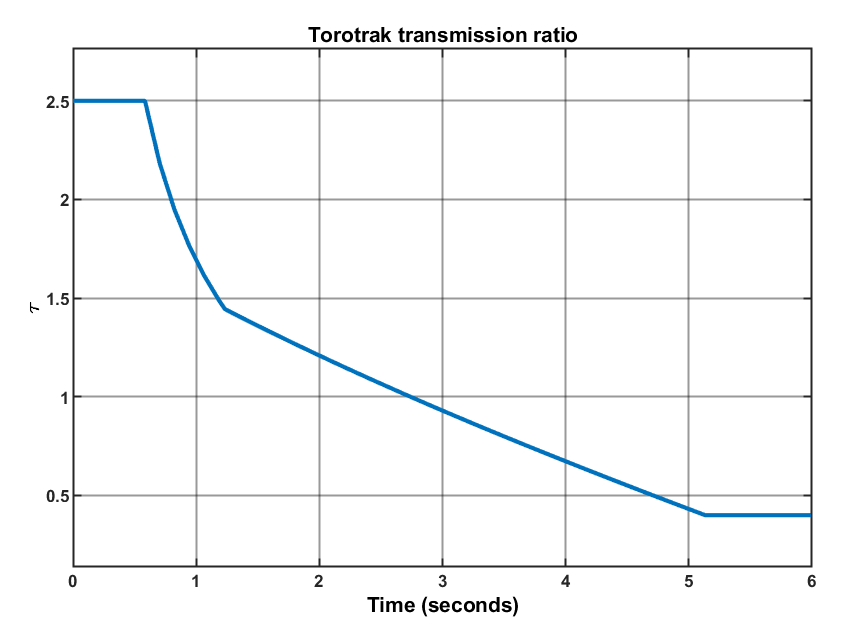
\includegraphics[width=.6\textwidth]{Images/Results_Dynamics/Charge/Torotrak_ratio.eps}
\caption{Behaviour of the transmission ratio of the Torotrak}
\label{fig: CVT_ratio_charge}
\end{figure}

In Fig.~\ref{fig: Vehicel_Vel_Charge} is represented the velocity of the vehicle in time. It can be noticed how there is a faster decrease of the speed in the first $1.2$ seconds, whereas after that the decrease in speed becomes almost linear\footnote{The presence of the aerodynamic force gives a small nonlinear contribution.}. 

The control effort is shown in Fig.~\ref{fig: Contro_Effort_Charge}. The control action contributes until the clutch is engaged, i.e. $0.6$ [s], then the behavior of the system depends only on the transmission ratio of the Torotrak. Of course, if one increases the proportional gain of the $PID$ controller (actually, the only used here), then the charge transient will reduce and the control effort will rise. This property of the control law can be exploited until reaching the physical upper limit of the actuator, which cannot bear huge magnitude in control, also because if the normal force applied to clutch plates $F_N$ is too high there could be problems and damages to the clutch itself.

\begin{figure}[H]
\centering
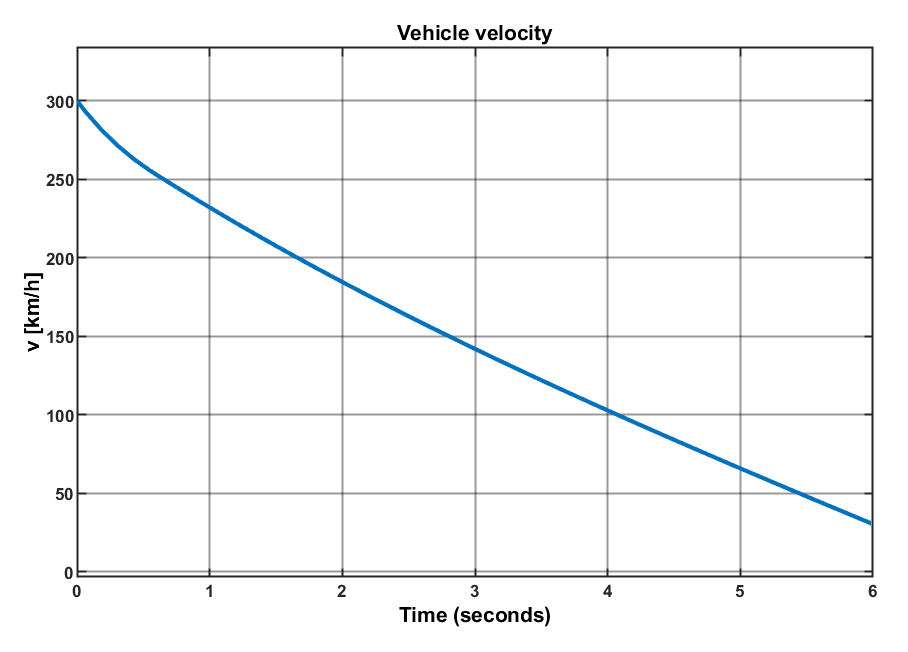
\includegraphics[width=.6\textwidth]{Images/Results_Dynamics/Charge/Vehicle_Vel.eps}
\caption{Velocity of the vehicle in the KERS charge phase}
\label{fig: Vehicel_Vel_Charge}
\end{figure}

\begin{figure}[H]
\centering
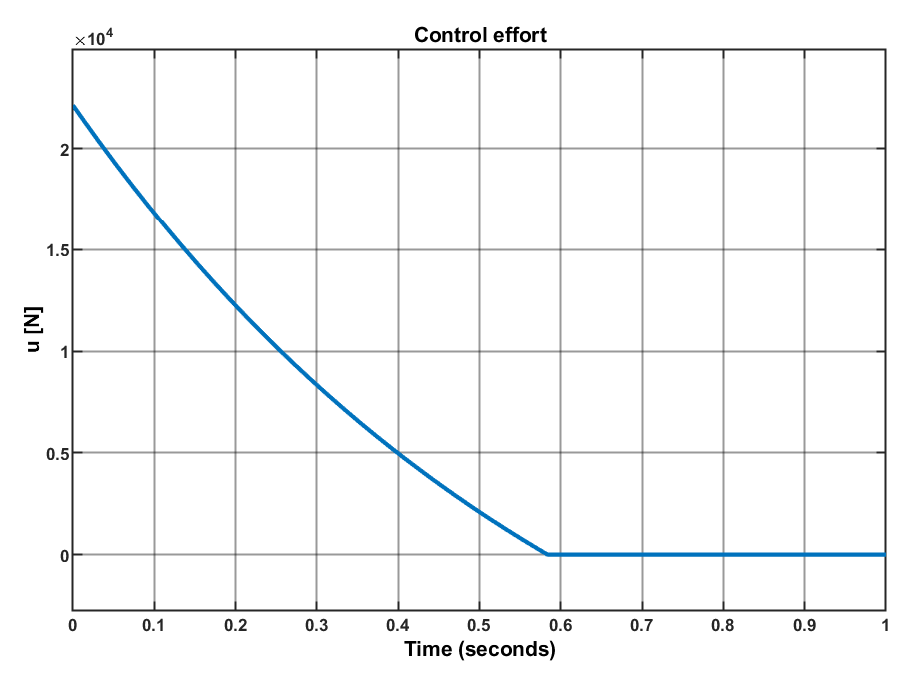
\includegraphics[width=.6\textwidth]{Images/Results_Dynamics/Charge/Control.eps}
\caption{Control effort in the KERS charge phase}
\label{fig: Contro_Effort_Charge}
\end{figure}

\subsubsection{KERS charge comparison}

Now, the results obtained in the charge phase are presented.

In Fig.~\ref{fig: Comparison_KERS_brake} it is shown how the presence of the KERS system is a great improvement during the deceleration phase and in particular at the beginning where the slope of the curve is very different. The presence of the KERS allows the car to have a deceleration gain of about $30$ [km/h] after $1$ [s].

In Fig.~\ref{fig: Comparison_KERS_brake_Control} it can be seen how the behavior of the velocity changes if, instead of applying a PID control, a constant control is applied with different magnitudes. In the latter situation the velocity decreases linearly which is not what happens in real scenarios where there is a strong initial deceleration but then it will become much slower in time.

\begin{figure}[H]
\centering
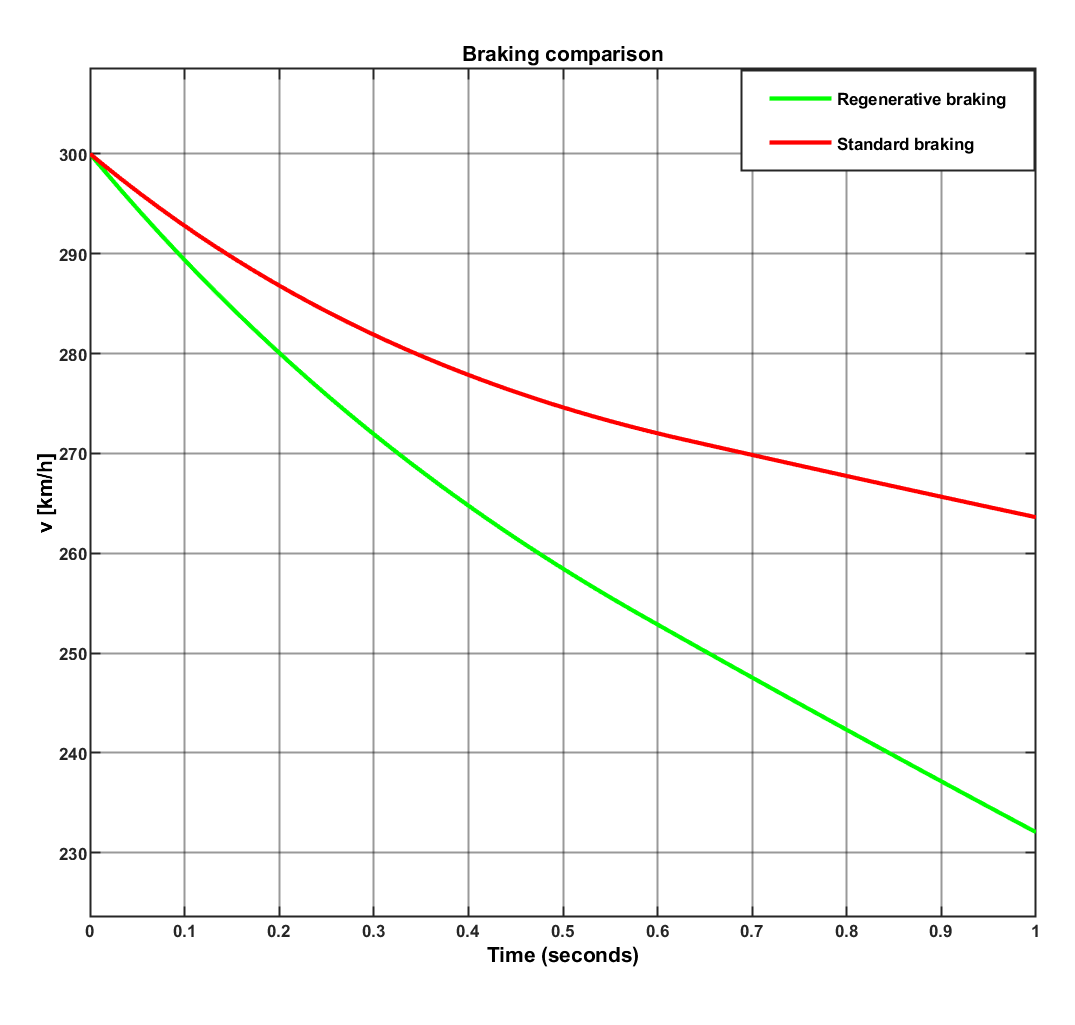
\includegraphics[width=.6\textwidth]{Images/Results_Dynamics/Charge_comparison/brake_kers_vs_nokers.eps}
\caption{Velocity of the vehicle during deceleration phase with and without KERS}
\label{fig: Comparison_KERS_brake}
\end{figure}

\begin{figure}[H]
\centering
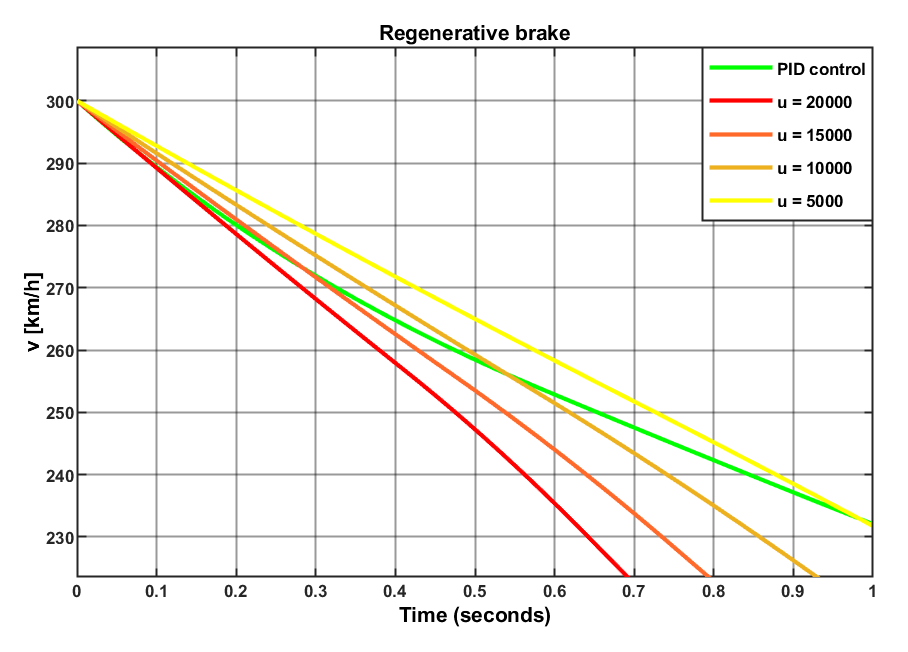
\includegraphics[width=.6\textwidth]{Images/Results_Dynamics/Charge_comparison/regenerative_brake_constantforce.eps}
\caption{Velocity comparison between a PID control and a constant force control}
\label{fig: Comparison_KERS_brake_Control}
\end{figure}

So the use of a PID control reflects well the behaviour of the car in the deceleration phase. 

In Fig.~\ref{fig: Comparison_KERS_Charge_PID_Prop} it is shown how the KERS charge behavior changes as we change the proportional gain of the controller. It can be seen that the choice of $K_p = 50$ which has been used in the previous section represents a good solution which is also a reasonable one in terms of time of charge and actuation stress. Instead in Fig.~\ref{fig: Comparison_KERS_Charge_Control} it can be seen the case in which a constant force or a PID control is applied. The greater the force the faster is the charge, however these behaviors are not so realistic because the time needed for a complete charge of the flywheel cannot be less than 1 second due to fact that really fast charge periods can deteriorate rapidly the KERS system.

\begin{figure}[H]
\centering
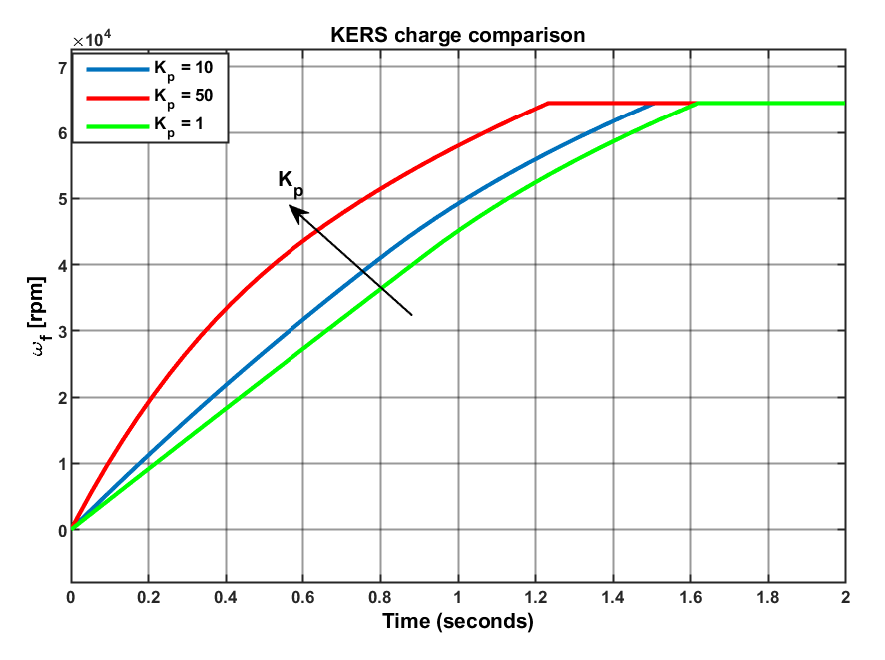
\includegraphics[width=.6\textwidth]{Images/Results_Dynamics/Charge_comparison/kers_charge_comp_PropGain.eps}
\caption{Comparison of KERS charge behaviour with different proportional gains}
\label{fig: Comparison_KERS_Charge_PID_Prop}
\end{figure}

\begin{figure}[H]
\centering
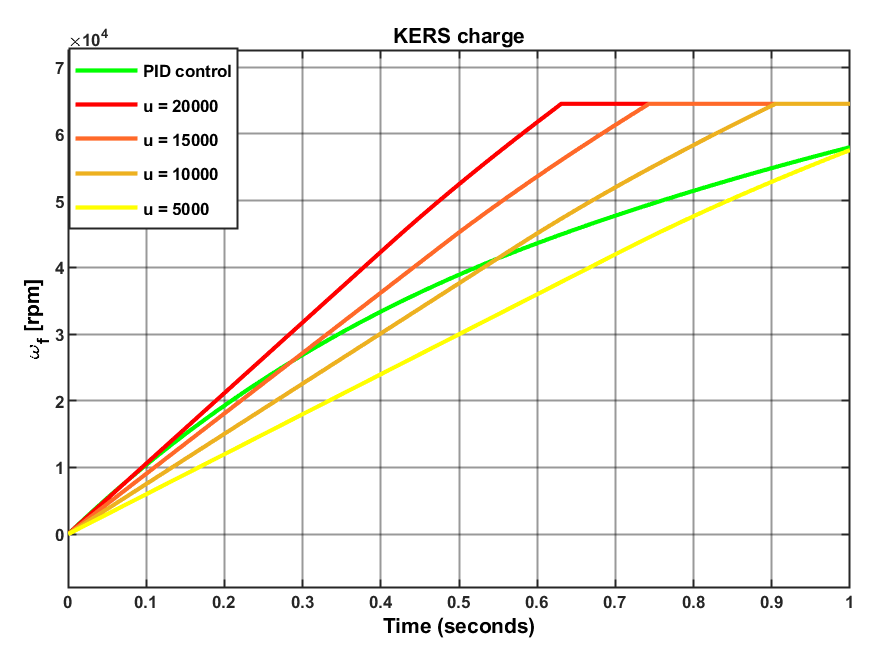
\includegraphics[width=.6\textwidth]{Images/Results_Dynamics/Charge_comparison/kers_charge_constantforce.eps}
\caption{Comparison of KERS charge behaviour between a PID control or a constant force control }
\label{fig: Comparison_KERS_Charge_Control}
\end{figure}

Below are presented some simulations in the case of a PI controller, so there is an additional integral term. In particular in Fig.~\ref{fig: Comparison_KERS_Charge_PI} it is shown how the greater this term is the faster is the charge of the flywheel. With $K_i = 1$ the behavior is the same as the one in Fig.~\ref{fig: ClutchVel}. Of course, a faster charge implies a greater control effort, in particular in the initial phase of the charge as it can be seen in Fig.\,\ref{fig: Comparison_Control_Effort_PI}. 

Since the velocity of the charge is more or less the same, it is preferable to choose the one which needs the less control effort to be performed, so the one with $K_i = 1$.

The last simulation which has been done is comparing the charge by changing the input of the controller, i.e. the feedback error signal. Until now the error was a linear one and was defined as the difference between the desired signal (trivially, zero) and the difference between the clutch angular velocities $\omega_{c,v}$ and $\omega_{c,k}$. This results into a final error of the type

\begin{equation}
e = \omega_{c,v} - \omega_{c,k}
\label{linear_error}
\end{equation}

In Fig.~\ref{fig: Comparison_KERS_charge_error} are presented the behaviors in the case of non--linear errors, in particular the square and the cube of the error in~\eqref{linear_error}. The controller which has been used is the PID with only a proportional gain $K_p = 10$ for the sake of simplicity. It can be seen how in this case the controller manages to perform the charge of the flywheel, however it is nearly instantaneous which is strongly unrealistic. So the PID controller is not a good choice if we want to analyze non--linear errors but we need a more complicated controller, possibly non--linear.

\begin{figure}[H]
\centering
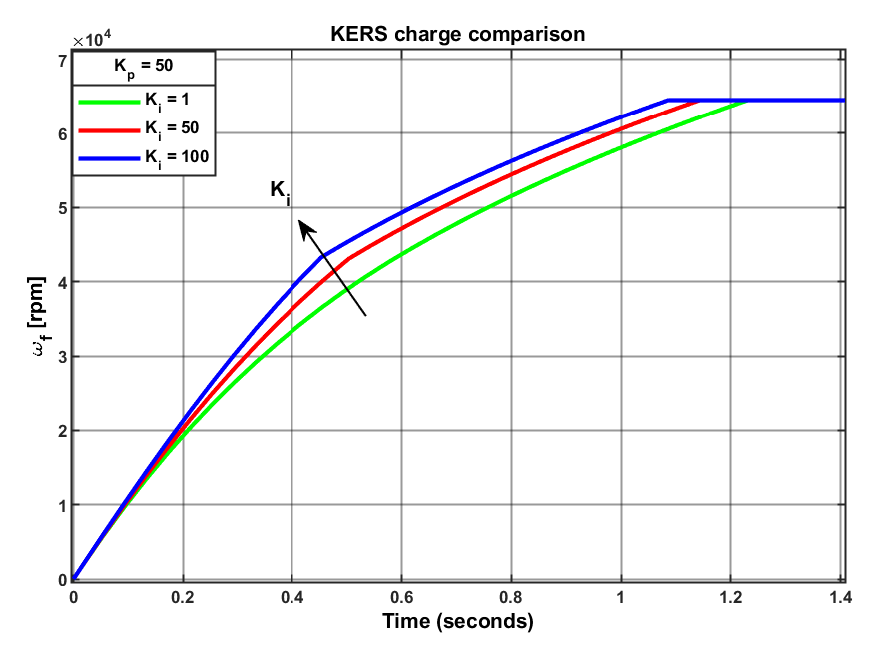
\includegraphics[width=.6\textwidth]{Images/Results_Dynamics/Charge_comparison/kers_charge_comp_IntGain.eps}
\caption{Comparison of KERS charge behaviour by using different values of the integral gain $K_i$}
\label{fig: Comparison_KERS_Charge_PI}
\end{figure}

\begin{figure}[H]
\centering
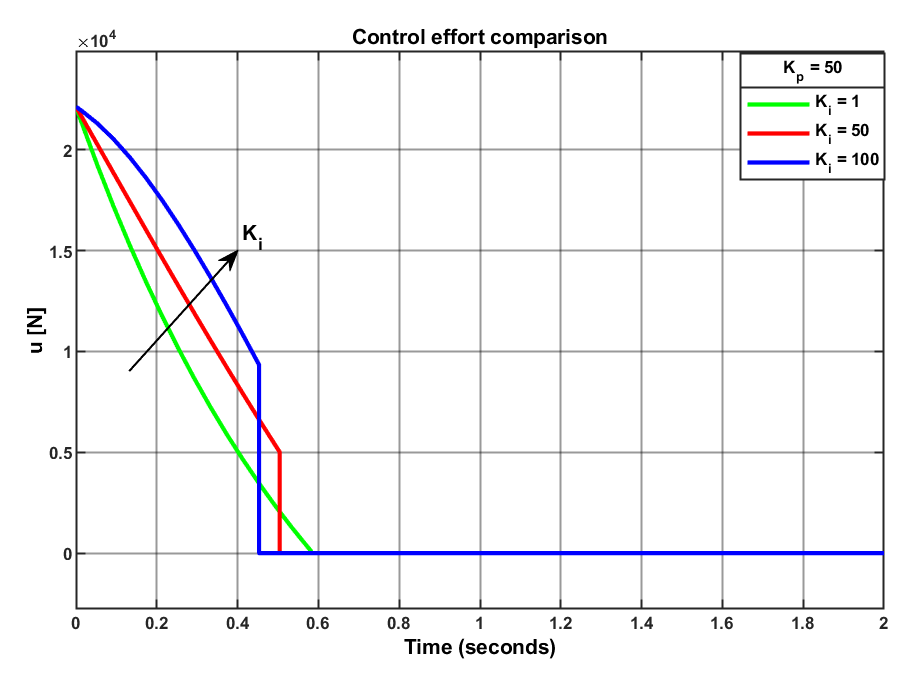
\includegraphics[width=.6\textwidth]{Images/Results_Dynamics/Charge_comparison/control_effort_charge_comp_IntGain.eps}
\caption{Comparison of control effort by using different values of the integral gain $K_i$}
\label{fig: Comparison_Control_Effort_PI}
\end{figure}

\begin{figure}[H]
\centering
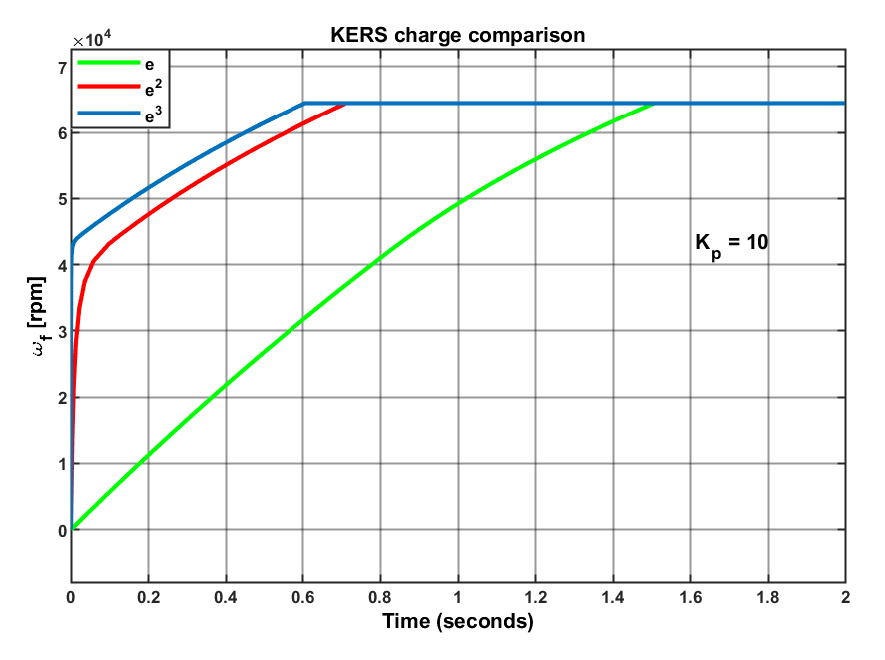
\includegraphics[width=.6\textwidth]{Images/Results_Dynamics/Charge_comparison/kers_charge_comp_controller.eps}
\caption{Comparison of KERS charge by using different expressions for the error}
\label{fig: Comparison_KERS_charge_error}
\end{figure}
%Codice per inserire le figure
\begin{comment}
\begin{figure}[H]
\centering
\includegraphics[width=.6\textwidth]{Charts/StepF1}
\caption{Step response of the closed--loop relative to $F_1$}
\label{StepF1}
\end{figure}
\end{comment}

\subsection{KERS Discharge}

In order to simulate the joint power contribution of both KERS and internal combustion engine, it is assumed the KERS to be fully charged at the maximum angular speed $ \omega_f^{max}=64000$ rpm. In order to appreciate the KERS contribution, it is assumed that the vehicle is proceeding at the maximum speed $ v = 315$ km/h. KERS is triggered at $30$ [s] so it starts to give power contribution from that instant on. This could be a realistic scenario because in Formula 1 steering wheel there is a button that the pilot could press in order to activate \textit{overtake modality} in order to have maximum acceleration contribution from KERS to overtake the opponent's vehicle. The control law used for the clutch engagement control is a PID with only proportional gain ($K_p = 50$). In Fig.\ref{fig: clutchengdis} it is shown the clutch engagement process.

\begin{figure}[H]
	\centering
	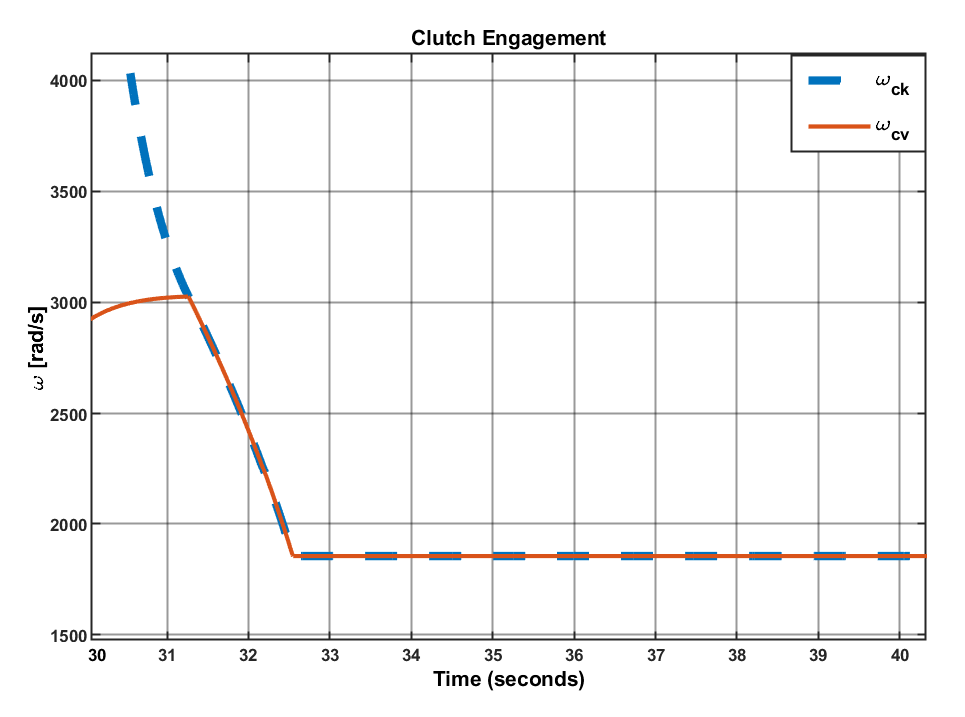
\includegraphics[width=.6\textwidth]{Images/Results_Dynamics/Discharge/Clutch_zoom.eps}
	\caption{Clutch engagement in KERS discharge scenario}
	\label{fig: clutchengdis}
\end{figure}

It is possible to clearly see how the two clutch plates start with angular velocities $\omega_{c,k} \neq \omega_{c,v}$. At the end of the transient the no--slipping condition is achieved and the engagement is completed. From the engagement instant on, the two plates will rotate at the same angular speed until the flywheel reaches $30\%$ of the maximum speed $w_f^{max}=64000$ rpm. At this point the KERS will be disengaged for efficiency reason (as it is also suggested in the patent taken as reference). The clutch plates engagement is controlled applying a suitable normal force to the clutch disks. From control viewpoint it is important to look at the control effort in order to check if the requested control action is feasible otherwise, when control action would be applied, the system would fail.

\begin{figure}[H]
	\centering
	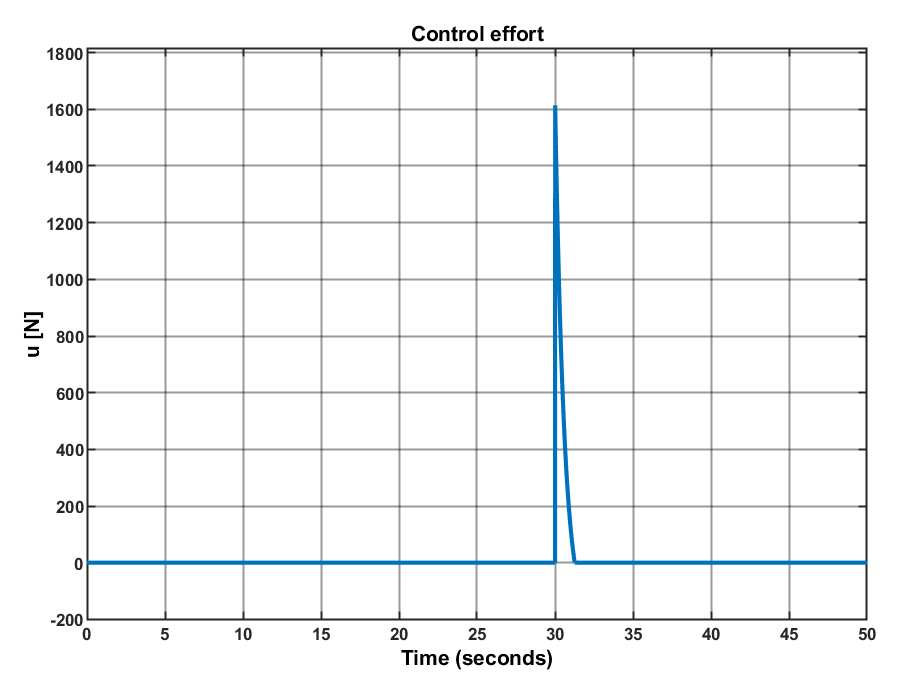
\includegraphics[width=.6\textwidth]{Images/Results_Dynamics/Discharge/Control.eps}
	\caption{Control}
	\label{fig: controldis}
\end{figure}

In Fig.~\ref{fig: controldis} control effort is shown and it is possible to see that the control acts only during the clutch engagement transient as it is expected. In fact, the orthogonal force over the plates aims to minimize the transient time, so once the transient end, the control action is null. Moreover, it is possible to note that the control effort is within the limits given by $u^{max} = 5000$ [N].

\begin{figure}[H]
	\centering
	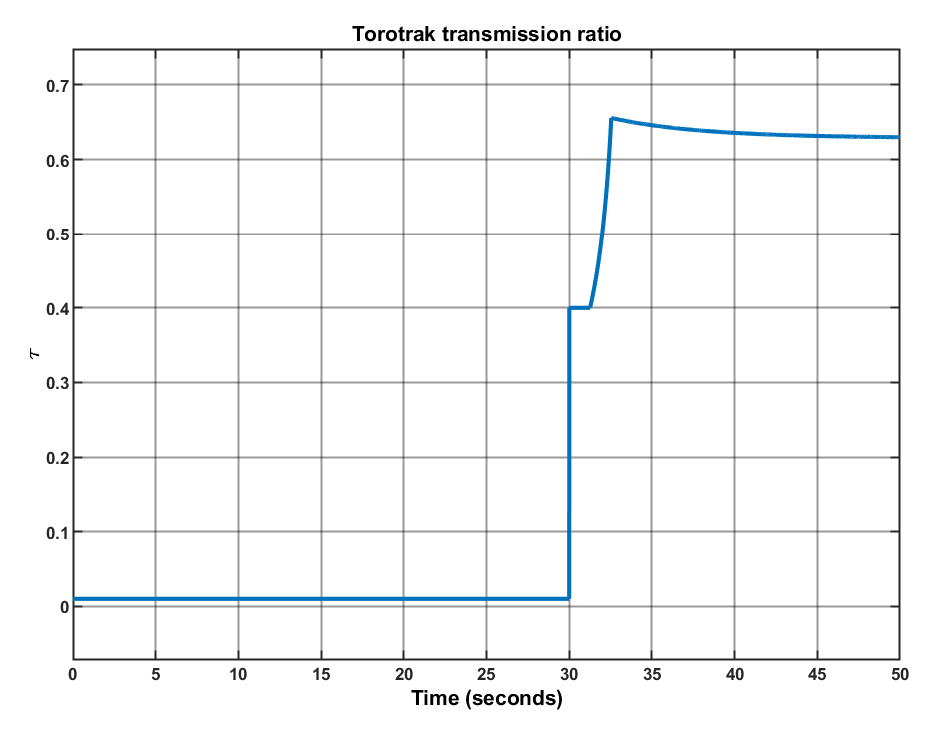
\includegraphics[width=.6\textwidth]{Images/Results_Dynamics/Discharge/Torotrak_ratio.eps}
	\caption{Torotrak ratio}
	\label{fig: tororatiodis}
\end{figure}

In Fig.~\ref{fig: tororatiodis} it is shown the Torotrak transmission ratio $\tau$. From the moment in which the KERS is triggered by the pilot at $30$s, for all the duration of the transient $\tau$ stays constant. Then it starts to increase in order to guarantee the correct power flow from KERS to the wheel after the clutch engagement transient. For the sake of completeness also the gearbox transmission ratio is shown in Fig.\,\ref{fig: gbratiodis}. It is possible to see how as the vehicle velocity increase the gear are shifted in order to have the best performances. In Fig.\,\ref{fig: kers vel plus vehicle vel} KERS and vehicle velocity profiles are shown.

\begin{figure}[H]
	\centering
	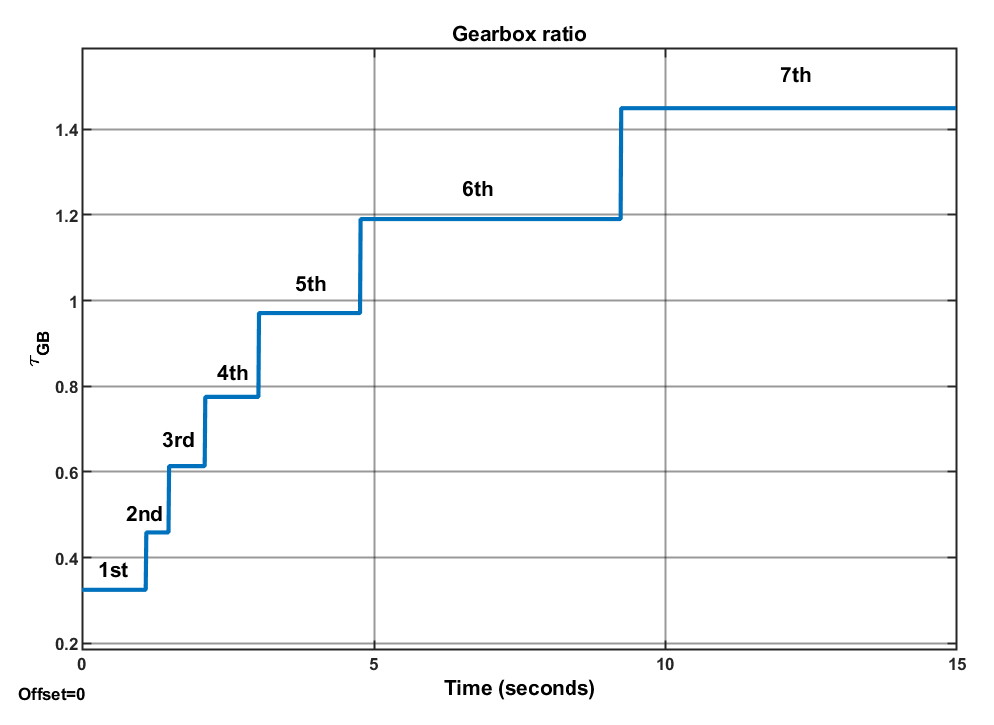
\includegraphics[width=.6\textwidth]{Images/Results_Dynamics/Discharge/Gearbox_ratio.eps}
	\caption{Gearbox ratio}
	\label{fig: gbratiodis}
\end{figure}
 
\begin{figure}[H]
	\centering
	\subfloat[][\emph{} \label{fig: kersveldiss}]
	{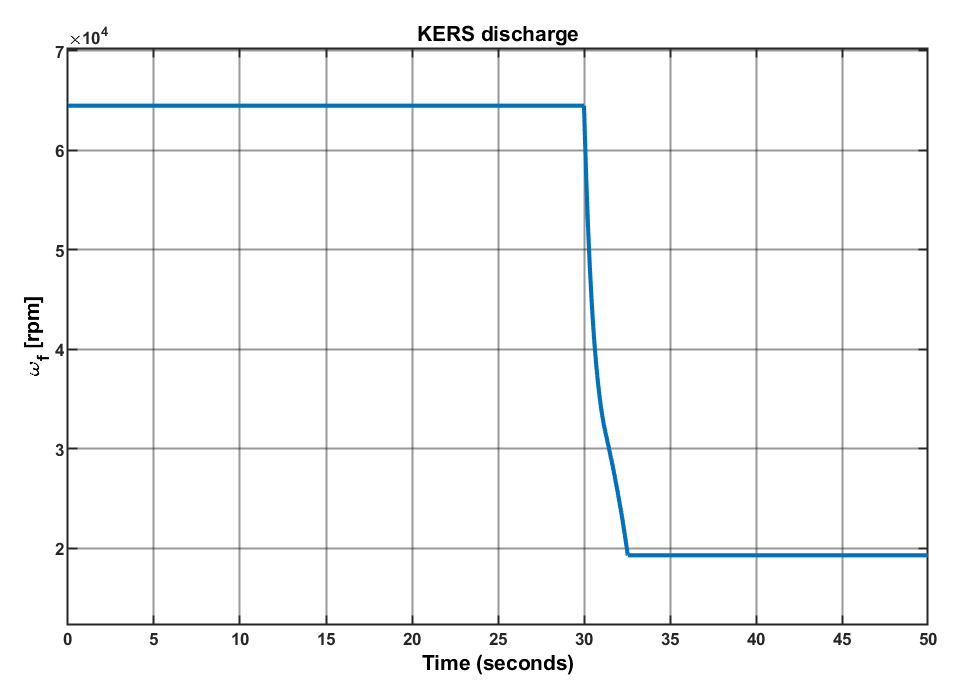
\includegraphics[width=.6\textwidth]{Images/Results_Dynamics/Discharge/KERS_Vel.eps}} \\
	\subfloat[][\emph{} \label{fig: vehicleveldisl}]
	{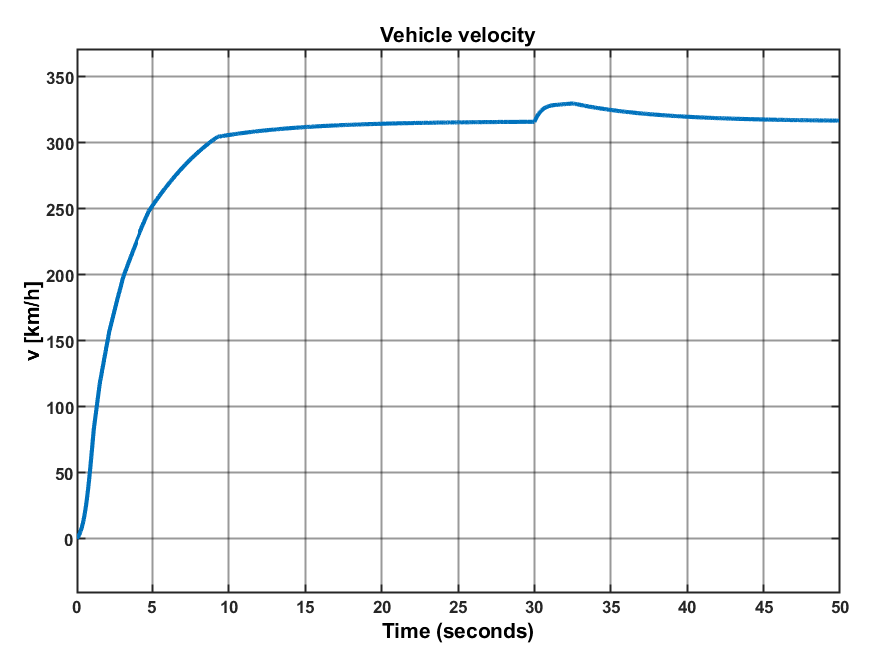
\includegraphics[width=.6\textwidth]{Images/Results_Dynamics/Discharge/Vehicle_Vel.eps}} \\
	\caption{Comparison between KERS velocity \protect\subref{fig: kersveldiss} and vehicle velocity \protect\subref{fig: vehicleveldisl}}
	\label{fig: kers vel plus vehicle vel}
\end{figure}

From these velocities profiles it is possible to see that as the flywheel angular speed decreases, the vehicle gains extra velocity. This confirms the power exchange from the flywheel to the wheels. As it is expected the KERS stops to give power contribution when it reaches $30\%$ of maximum speed.

\subsubsection{KERS discharge comparison}

In order to analyze the importance of KERS contribution to improve sport performances it may be interesting to look at vehicle velocity profile and to compare the case in which the KERS is present and it gives a joint contribution together with the engine to the vehicle and the case in which the KERS is not present.

\begin{figure}[H]
	\centering
	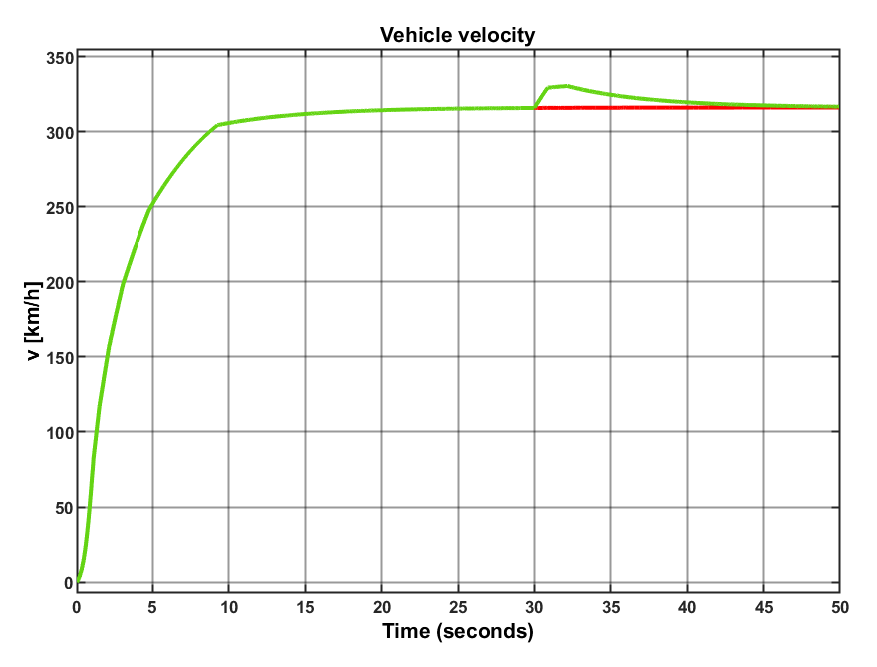
\includegraphics[width=.6\textwidth]{Images/Results_Dynamics/Discharge_comparison/acceleration_kers_vs_nokers.eps}
	\caption{Comparison between vehicle's velocity profile when KERS is active and when do not.}
	\label{fig: k vs nok}
\end{figure}

It is clear from Fig.~\ref{fig: k vs nok} that, while using KERS, it is possible to reach velocities that otherwise, with the only engine contribution, it would be impossible to reach. Once the importance of the KERS is confirmed through simulation data, then it could be interesting to investigate how different control strategies affect performances.

\begin{figure}[H]
	\centering
	\subfloat[][\emph{} \label{fig: varyPdisdis}]
	{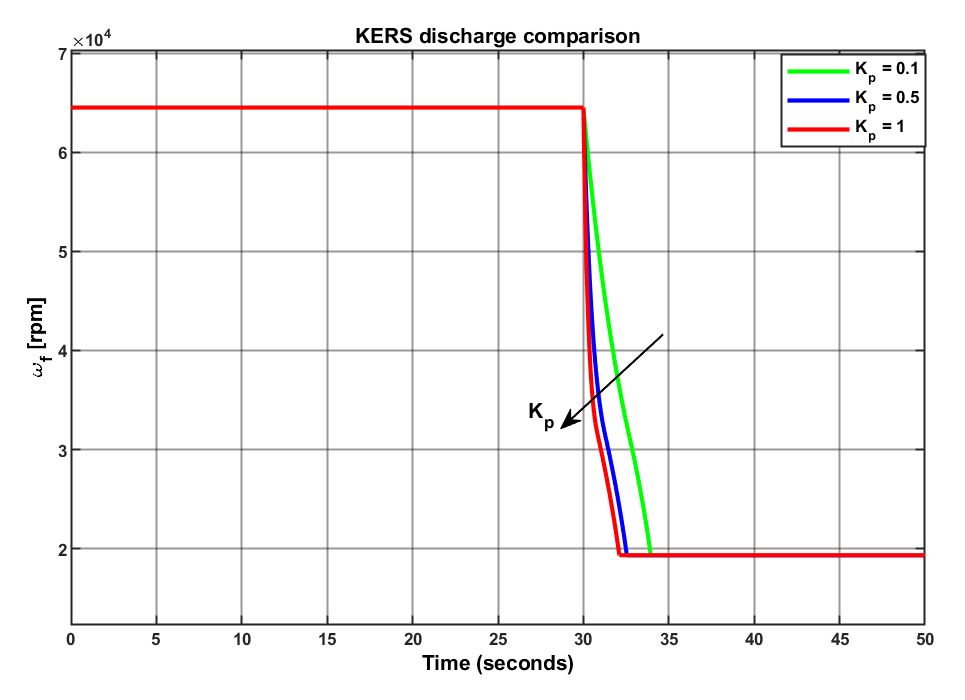
\includegraphics[width=.6\textwidth]{Images/Results_Dynamics/Discharge_comparison/kers_discharge_comp_PropGain.eps}} \\
	\subfloat[][\emph{} \label{fig: varyPaccdis}]
	{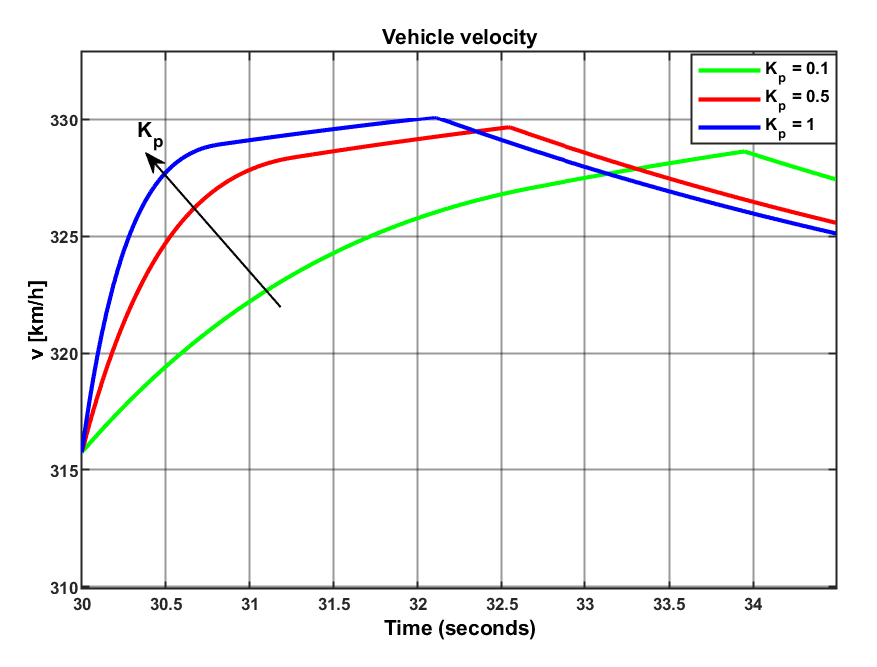
\includegraphics[width=.6\textwidth]{Images/Results_Dynamics/Discharge_comparison/vehicle_acc_comp_PropGain.eps}} \\
	\caption{Comparison between KERS velocity \protect\subref{fig: varyPdisdis} and vehicle velocity in discharge scenario when proportional gain is changed \protect\subref{fig: varyPaccdis}}
	\label{fig: kers vel plus vehicle vel comp}
\end{figure}

In Fig.\,\ref{fig: kers vel plus vehicle vel comp} it is shown how KERS discharge process changes when PID proportional term changes. The higher $K_p$ the faster is the discharge and the higher the peak vehicle velocity.

\begin{figure}[H]
	\centering
	\subfloat[][\emph{} \label{fig: kforcedisdis}]
	{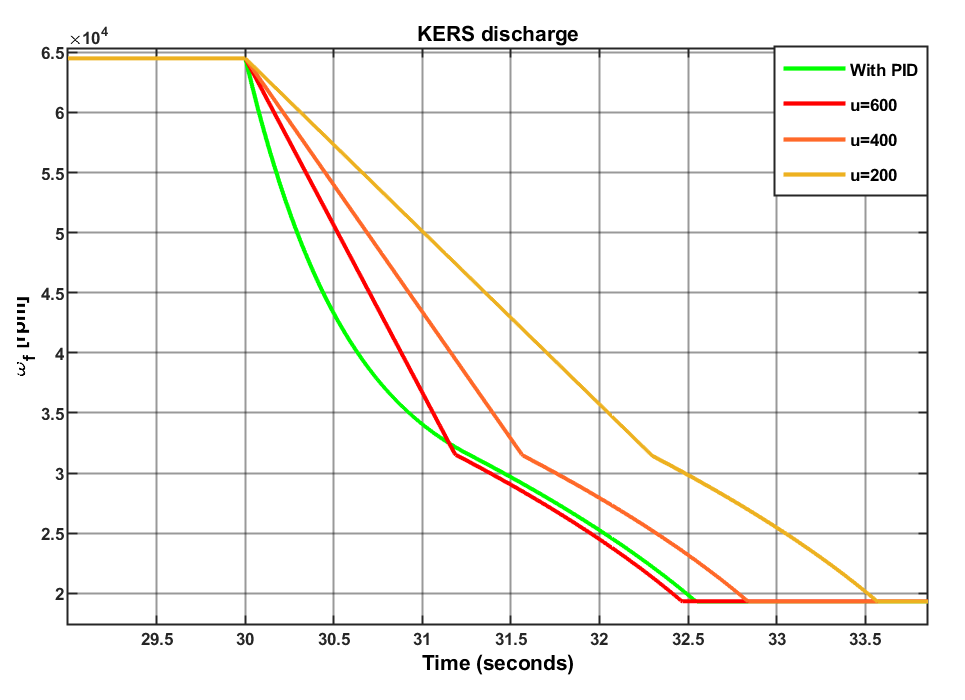
\includegraphics[width=.6\textwidth]{Images/Results_Dynamics/Discharge_comparison/kers_discharge_constantforce.eps}} \\
	\subfloat[][\emph{} \label{fig: kforceaccdis}]
	{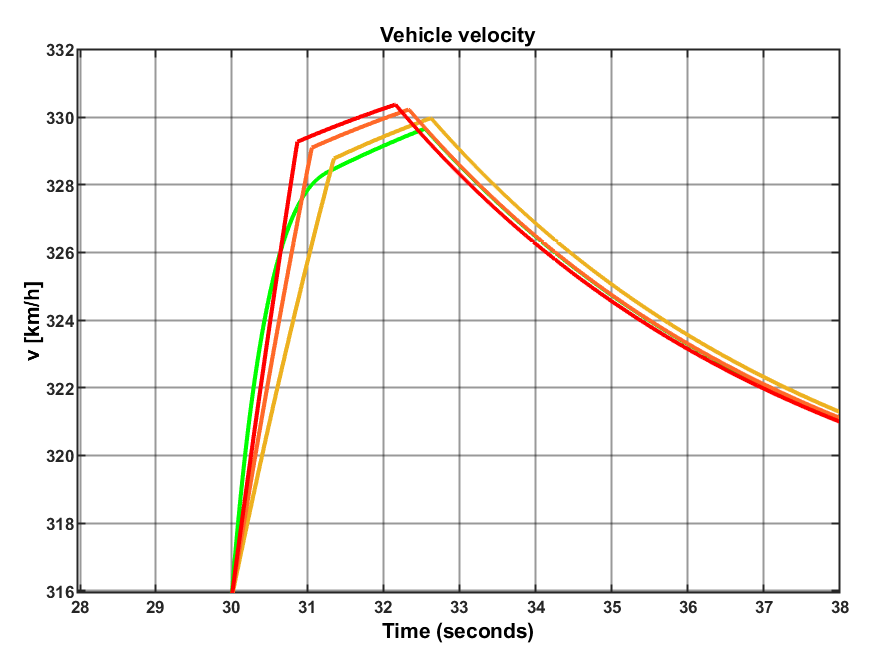
\includegraphics[width=.6\textwidth]{Images/Results_Dynamics/Discharge_comparison/regenerative_acc_constantforce.eps}} \\
	\caption{Comparison between KERS velocity \protect\subref{fig: kforcedisdis} and vehicle velocity  \protect\subref{fig: varyPaccdis} in discharge scenario when constant force acting on clutch's plates is changed.}
	\label{fig: kforcediscomp}
\end{figure}

Until now it was only considered PID strategy with only proportional component for the clutch engagement control. If clutch plates are engaged with constant forces (Fig.~\ref{fig: kforcediscomp}), one can appreciate that, in order to have results similar or better with respect to the PID, higher force is needed. The higher is the force the faster is the discharge and the higher is the maximum velocity reached by the vehicle. 

\newpage

\section{Conclusions}

In this work a particular type of Kinetic Energy Recovery System (KERS) was studied. Different implementations widely used in literature and in real applications were taken into account and mechanical KERS was chosen to be investigated in more detail. MKERS turns out to have lesser cost than the other ones and it is preferable in the competition scenario, working with high velocity and relatively small car mass. Moreover, MKERS has a low cost with respect to the regenerative systems used for commercial vehicles or transportation systems (buses, trucks, and son on). 

The patent used as reference is the one developed by Flybrid\textsuperscript\textregistered. The driveline is the one typical of a MKERS, with the special possibility to select eight fixed gear ratios which link the flywheel to the clutch.

Analysis, modeling, simulation and control of KERS was developed in this work. First, static analysis was performed. This kind of study allows to state the performance of the regenerative braking without taking into account the whole dynamics of the process. Hence, the static analysis can be useful in order to evaluate the properties of the transmission line, highlighting the benefits and the disadvantages of using certain values for the limits of the CVT or, equivalently, for the final gearbox. 

Afterwards, a dynamic model was considered. It has been built starting from a lagrangian formulation through which a conservative model has been obtained. After this, in order to complete the dynamics in the two phases (charge and discharge) the non--conservative fields have been included, such as braking, aerodynamic friction and clutch engagement dynamics. The latter allows, by means of an active system, to introduce a user--defined control action.

The dynamic model has been validated according to the static analysis. All the simulations was implemented in Simulink and different feedback control strategies were applied to the clutch engagement process like PID and constant forces. 

The results show that both KERS charge and discharge can be improved when using a large constant normal force or when using in a proper way a pure proportional controller, whose input is the clutch engagement error, i.e. the difference between the two velocities of the clutch plates.

Eventually, it can be concluded that MKERS, together with the engine contribution, gives a high speed--up for several seconds to the F1 vehicle also when it has already reached its maximum velocity. This speed--up performance can be significantly improved with an active clutch engagement, because the vehicle receives the amount of energy stored in the flywheel in shorter time.  


%Codice per inserire il codice
\begin{comment}
\vspace{4cm}
	This is a fancy in--line code
	\singlespacing
	\begin{Verbatim}[tabsize = 4, frame = lines, numbers = left]
	code_here...
	code_here...
	code_here...
	\end{Verbatim}
	\onehalfspacing
\end{comment}

\newpage

\begin{thebibliography}{60}
	
	%%%
	
	%GENERAL STRUCTURE FOR THE BIBLIOGRAPHY
	
	%Cognome, Nome appuntato, (Anno), Nome del paper o del libro, Editrice o rivista, città (Stato), pagine.
	
	%Esempio
	%Kapoor R., Parveen C. M., (2013), \textit{Comparative %Study on Various KERS}, Proceedings of the World Congress %on Engineering 2013 Vol III, London.
	
	%%%
	\bibitem{a}
	Chibulka J., (2009), \textit{Kinetic Energy Recovery system by means of Flywheel Energy storage device}, Advanced Engineering, vol. 3, issue 1, pp. 27-38.
	
	\bibitem{b}
	Chicurel R., (2009),  \textit{A Compromise Solution for Energy Recovery in Vehicle Braking}, Energy, vol.24, pp. 1029-1034.
	
	\bibitem{c}
	Harb A., (2011), \textit{Energy harvesting: State-of-the-art}, 
	Renewable energy, vol. 36, pp. 2641-2654, 2011.
	
	\bibitem{d}
	Baer K. et al., (2020) \textit{Robustness and performance evaluations for simulation-based 		control and component parameter optimization for a series hydraulic hybrid vehicle}, Engineering Optimization, vol. 52, no. 3, pp. 446–464.	
	
	\bibitem{e}
	Kim Y. J. et al., (2007), \textit{Simulation Study of a Series Hydraulic Hybrid Propulsion System for a Light Truck}, SAE International.
	
	\bibitem{f}
	Shan M., (2009), \textit{Modelling and Control Strategy for Series Hydraulic Hybrid Vehicles}, PhD thesis.
	
	\bibitem{g}
	Nishanth D., Mathews T., (2013), \textit{Flywheel based Kinetic Energy Recovery System(KERS) 	    integrated in vehicles}, International Journal of Engineering Science and Technology (IJEST), vol. 5 no.09.
	
	\bibitem{h}
	Pipitone E., Vitale G., (2020), \textit{A regenerative braking system for internal combustion engine vehicles using supercapacitors as energy storage 		elements-Part 1 and 2: System analysis and modelling}, Journal of Power Sources 448, Palermo (Italy).     	
	
	\bibitem{i}
	Itani K., De Bernardinis A., Khatir Z, Jammal A., (2017),  							\textit{Comparative analysis of two hybrid energy storage systems used in a 		two front wheel driven electric vehicle during extreme start-up and 				regenerative braking operations},  Energy Conversion and Management, Beirut 		(Lebanon), pp. 69-87.
	
	\bibitem{l}
	Kapoor R., Parveen C. M., (2013), \textit{Comparative Study on Various KERS},   	Proceedings of the World Congress on Engineering 2013 Vol III, London.
	
	\bibitem{m}
	Hui S., Lifu Y., Junqing J., (2010), \textit{Hydraulic/electric synergy   	 	    system (HESS) design for heavy hybrid vehicles}, Energy 35, pp. 5328--5335.
	
	\bibitem{n}
	Jones D. R., (2016), \textit{Kinetic energy recovery system},
	UK Patent.  
	
	\bibitem{o}
	Lee H., Kim H., (2003), \textit{CVT Ratio Control for Improvement of Fuel Economy
	by Considering Powertrain Response Lag}, KSME International Journal, vol. 17, no. 11, pp. 1725--1731. 
	
	\bibitem{clutch}
	Glielmo L., Vasca F., (2000), \textit{Engagement Control for Automotive Dry Clutch}, Proceedings of the American Control Conference, Chicago, Illinois, pp. 1016--1017.
\end{thebibliography}

\end{document}
